% !TEX program = xelatex
% ============================================================
%  机器学习 · 讲义  第二讲：线性判别分析
%  海军深蓝 · 经典学术版式
%  编译：xelatex 02_lda.tex
%        （无 .aux 时连跑三遍；已有中间文件时两遍即可）
%        或直接用 latexmk -xelatex 02_lda.tex
% ============================================================
\documentclass[11pt,a4paper,fontset=windows,zihao=-4]{ctexart}

% ---------- 版面 ----------
\usepackage{geometry}
\geometry{a4paper,left=2.55cm,right=2.55cm,top=2.55cm,bottom=2.45cm,
  headheight=18pt,headsep=0.52cm,footskip=0.95cm,
  marginparsep=0.40cm,marginparwidth=2.10cm}

% ---------- 数学与字体 ----------
\usepackage{amsmath,amssymb,amsthm,mathtools}
\usepackage{newpxtext,newpxmath}
\usepackage{microtype}

% ---------- 颜色 ----------
\usepackage[table]{xcolor}
\definecolor{navy}{HTML}{0B2545}      % 海军深蓝（主色）
\definecolor{navy2}{HTML}{33587A}     % 次级蓝
\definecolor{steel}{HTML}{4A6478}     % 灰蓝
\definecolor{grey}{HTML}{6B7280}      % 中性灰
\definecolor{mist}{HTML}{F4F6F9}      % 极浅蓝灰（底色）
\definecolor{gold}{HTML}{8A6A3B}      % 暗金（仅用于提示）
\definecolor{goldlight}{HTML}{C6A15B} % 亮金（深蓝底上的金线）

% ---------- 表格与列表 ----------
\usepackage{booktabs}
\usepackage{array}
\usepackage{multirow}
\usepackage{enumitem}
\setlist[itemize]{leftmargin=1.6em,topsep=0.45em,itemsep=0.28em,parsep=0pt}
\setlist[enumerate]{leftmargin=2.0em,topsep=0.45em,itemsep=0.28em,parsep=0pt}

% ---------- 图形 ----------
\usepackage{tikz}
\usetikzlibrary{calc,positioning,arrows.meta,decorations.pathreplacing,
  patterns,backgrounds,fit,shapes.geometric}
\usepackage{pgfplots}
\pgfplotsset{compat=1.18}

% ---------- 彩色框 ----------
\usepackage[most]{tcolorbox}

% ---------- 页眉页脚 ----------
\usepackage{fancyhdr}
\usepackage{titlesec}
\usepackage{caption}
\usepackage{marginnote}
\usepackage{tocloft}

% ---------- 超链接 ----------
\usepackage[colorlinks=true,linkcolor=navy,urlcolor=steel,citecolor=navy,
  bookmarksnumbered=true]{hyperref}
\hypersetup{
  pdftitle={机器学习·讲义（第二讲）：线性判别分析},
  pdfauthor={小算},
  pdfsubject={Fisher 准则、散布矩阵与判别函数},
  pdfkeywords={线性判别分析, LDA, Fisher 判别, 散布矩阵, 广义特征值, 降维, GDA}
}

% ============================================================
%  数学宏
% ============================================================
\newcommand{\R}{\mathbb{R}}
\newcommand{\bX}{\mathbf{X}}
\newcommand{\by}{\mathbf{y}}
\newcommand{\bw}{\mathbf{w}}
\newcommand{\bx}{\mathbf{x}}
\newcommand{\bz}{\mathbf{z}}
\newcommand{\be}{\mathbf{e}}
\newcommand{\ba}{\mathbf{a}}
\newcommand{\bb}{\mathbf{b}}
\newcommand{\bu}{\mathbf{u}}
\newcommand{\bA}{\mathbf{A}}
\newcommand{\bB}{\mathbf{B}}
\newcommand{\bQ}{\mathbf{Q}}
\newcommand{\bR}{\mathbf{R}}
\newcommand{\bS}{\mathbf{S}}
\newcommand{\bT}{\mathbf{T}}
\newcommand{\bmu}{\boldsymbol{\mu}}
\newcommand{\bv}{\mathbf{v}}
\newcommand{\bPhi}{\boldsymbol{\Phi}}
\newcommand{\bI}{\mathbf{I}}
\newcommand{\bH}{\mathbf{H}}
\newcommand{\bV}{\mathbf{V}}
\newcommand{\bU}{\mathbf{U}}
\newcommand{\bW}{\mathbf{W}}
\newcommand{\bSigma}{\boldsymbol{\Sigma}}
\newcommand{\bLambda}{\boldsymbol{\Lambda}}
\newcommand{\bepsilon}{\boldsymbol{\epsilon}}
\newcommand{\btheta}{\boldsymbol{\theta}}
\newcommand{\bphi}{\boldsymbol{\phi}}
\newcommand{\bdelta}{\boldsymbol{\delta}}
\newcommand{\bL}{\mathbf{L}}
\newcommand{\bM}{\mathbf{M}}
\newcommand{\bzero}{\mathbf{0}}
\newcommand{\tp}{^{\top}}
\newcommand{\norm}[1]{\lVert #1\rVert}
\newcommand{\abs}[1]{\lvert #1\rvert}
\DeclareMathOperator*{\argmin}{arg\,min}
\DeclareMathOperator*{\argmax}{arg\,max}
\DeclareMathOperator{\tr}{tr}
\DeclareMathOperator{\rank}{rank}
\DeclareMathOperator{\Col}{Col}
\DeclareMathOperator{\Span}{Span}
\DeclareMathOperator{\sign}{sign}
\DeclareMathOperator{\Var}{Var}
\DeclareMathOperator{\Cov}{Cov}
\DeclareMathOperator{\diag}{diag}
\newcommand{\dd}{\mathrm{d}}

% ============================================================
%  版式细节
% ============================================================
\linespread{1.30}
\setlength{\parskip}{0.24em}
\setlength{\parindent}{2em}

% 章节样式
\ctexset{
  section/name={},
  section/number=\arabic{section},
}
\titleformat{\section}[block]
  {\normalfont\sffamily\Large\bfseries\color{navy}}
  {\colorbox{navy}{\makebox[1.55em][c]{\color{white}\thesection}}\hspace{0.75em}}{0pt}{}
  [\vspace{0.30em}{\color{navy!30}\titlerule[0.7pt]}]
\titlespacing*{\section}{0pt}{2.4ex plus 1.0ex minus 0.4ex}{1.5ex}

\titleformat{\subsection}[hang]
  {\normalfont\sffamily\large\bfseries\color{navy!88}}
  {\thesubsection}{0.65em}{}
\titlespacing*{\subsection}{0pt}{1.8ex plus 0.6ex}{0.8ex}

\titleformat{\subsubsection}[runin]
  {\normalfont\sffamily\bfseries\color{navy!80}}
  {}{0pt}{}
\titlespacing*{\subsubsection}{0pt}{1.2ex plus 0.4ex}{0.6em}

\titleformat{\paragraph}[runin]
  {\normalfont\sffamily\bfseries\color{navy!88}}
  {}{0pt}{}
\titlespacing*{\paragraph}{0pt}{1.05ex plus 0.35ex}{0.55em}

% 页眉页脚
\pagestyle{fancy}
\fancyhf{}
\renewcommand{\headrulewidth}{0.5pt}
\renewcommand{\headrule}{{\color{navy!40}%
  \hrule height \headrulewidth width \headwidth}}
\fancyhead[L]{\sffamily\footnotesize\color{steel}机器学习\,·\,讲义}
\fancyhead[R]{\sffamily\footnotesize\color{steel}\leftmark}
\fancyfoot[C]{\sffamily\footnotesize\color{navy}\thepage}
\renewcommand{\sectionmark}[1]{\markboth{\thesection\quad #1}{}}
\fancypagestyle{plain}{%
  \fancyhf{}\renewcommand{\headrulewidth}{0pt}%
  \fancyfoot[C]{\sffamily\footnotesize\color{navy}\thepage}}

% 图表标题
\captionsetup{font={small},labelfont={bf,sf,color=navy},labelsep=quad,
  justification=centering,skip=6pt}

% 目录（手工排版标题，避免 \leftmark 捕获颜色命令）
\renewcommand{\contentsname}{目\quad 录}
\makeatletter
\renewcommand{\tableofcontents}{%
  \par\begingroup
    \sffamily\Large\bfseries\color{navy}目\quad 录\par
  \endgroup
  \vspace{0.85em}
  \setlength{\parskip}{0pt}%
  \@starttoc{toc}%
}
\makeatother

% 目录条目样式
\renewcommand{\cftsecfont}{\footnotesize\sffamily\bfseries\color{navy}}
\renewcommand{\cftsecpagefont}{\footnotesize\sffamily\bfseries\color{navy}}
\renewcommand{\cftsubsecfont}{\footnotesize\color{navy!85}}
\renewcommand{\cftsubsecpagefont}{\footnotesize\color{navy!85}}
\renewcommand{\cftsubsubsecfont}{\color{steel}}
\renewcommand{\cftsubsubsecpagefont}{\color{steel}}
\renewcommand{\cftsecleader}{\cftdotfill{\cftdotsep}}
\renewcommand{\cftsubsecleader}{\cftdotfill{\cftdotsep}}
\renewcommand{\cftsubsubsecleader}{\cftdotfill{\cftdotsep}}
\setlength{\cftsecnumwidth}{1.9em}
\setlength{\cftsubsecnumwidth}{2.5em}
\setlength{\cftsubsubsecnumwidth}{3.4em}
\setlength{\cftbeforesecskip}{4.0pt}
\setlength{\cftbeforesubsecskip}{0.2pt}
\setlength{\cftbeforesubsubsecskip}{0pt}
\renewcommand{\cftsecaftersnum}{\hspace{0.55em}}
\renewcommand{\cftsubsecaftersnum}{\hspace{0.4em}}
\renewcommand{\cftsubsubsecaftersnum}{\hspace{0.35em}}

% ============================================================
%  提示框样式
% ============================================================
\tcbset{
  basebox/.style={
    enhanced, breakable, sharp corners,
    boxrule=0pt, leftrule=2.2pt, arc=0pt, outer arc=0pt,
    left=0.9em, right=0.9em, top=0.45em, bottom=0.62em,
    before skip=0.85em, after skip=0.85em,
    before upper={\parindent=0pt\parskip=0.35em},
    fonttitle=\sffamily\bfseries\small,
    coltitle=navy, titlerule=0.35pt,
    toptitle=0.32em, bottomtitle=0.5em,
  }
}
\newtcolorbox[auto counter,number within=section]{dfn}[1][]{%
  basebox, colframe=navy, colback=mist, colbacktitle=mist,
  title={定义~\thetcbcounter\quad\textcolor{navy!45}{\textbar}\quad\textcolor{navy}{#1}}}
\newtcolorbox[auto counter,number within=section]{thm}[1][]{%
  basebox, colframe=navy, colback=white, colbacktitle=white,
  title={定理~\thetcbcounter\quad\textcolor{navy!45}{\textbar}\quad\textcolor{navy}{#1}}}
\newtcolorbox[auto counter,number within=section]{prop}[1][]{%
  basebox, colframe=navy2, colback=white, colbacktitle=white,
  title={命题~\thetcbcounter\quad\textcolor{navy!45}{\textbar}\quad\textcolor{navy}{#1}}}
\newtcolorbox[auto counter,number within=section]{exm}[1][]{%
  basebox, colframe=steel, colback=white, colbacktitle=white,
  title={例~\thetcbcounter\quad\textcolor{navy!45}{\textbar}\quad\textcolor{steel}{#1}}}
\newtcolorbox{add}[1][]{%
  basebox, colframe=steel, colback=mist, colbacktitle=mist,
  title={\textcolor{steel}{补充}\quad\textcolor{steel!45}{\textbar}\quad\textcolor{steel}{#1}}}
\newtcolorbox{warn}[1][]{%
  basebox, colframe=gold, colback=gold!4, colbacktitle=gold!4,
  title={\textcolor{gold}{注意}\quad\textcolor{gold!55}{\textbar}\quad\textcolor{gold}{#1}}}
\newtcolorbox{keybox}[1][]{%
  enhanced, breakable, sharp corners, boxrule=0.55pt,
  colframe=navy!55, colback=navy!3, colbacktitle=navy!3,
  left=0.9em, right=0.9em, top=0.45em, bottom=0.62em,
  before skip=1.0em, after skip=1.0em,
  before upper={\parindent=0pt\parskip=0.35em},
  fonttitle=\sffamily\bfseries\small, coltitle=navy,
  titlerule=0.35pt, toptitle=0.3em, bottomtitle=0.5em,
  title={\textcolor{navy}{#1}}}

% 边注
\renewcommand*{\marginfont}{\footnotesize\color{steel}}
\setlength{\marginparpush}{6pt}

% 常用小工具
\newcommand{\hl}[1]{\textcolor{navy}{\textbf{#1}}}
\newcommand{\tabhead}{\sffamily\bfseries\color{navy}}
% 图上用的极简样式
\tikzset{
  cls1/.style={fill=navy,draw=none},
  cls2/.style={fill=goldlight,draw=none},
  frame/.style={draw=steel!30,line width=0.4pt},
  axisar/.style={->,steel!55,line width=0.5pt},
  lab/.style={font=\scriptsize,text=steel,inner sep=2pt},
}

\begin{document}

% ============================================================
%  封面 · 目录 · 导读
% ============================================================

\begin{titlepage}
\thispagestyle{empty}
\raggedright
% ---- 顶部深蓝色块 + 金色分隔线 + 两类散点与判别方向 ----
\begin{tikzpicture}[remember picture, overlay]
  \fill[navy] (current page.north west) rectangle ([yshift=-12.30cm]current page.north east);
  \fill[goldlight] ([yshift=-12.30cm]current page.north west)
        rectangle ([yshift=-12.37cm]current page.north east);
  % 右侧：两类样本 + Fisher 方向（正文例题的真实解）
  \begin{scope}[shift={([xshift=12.30cm,yshift=-10.28cm]current page.north west)}]
    % 轴框（极淡）
    \draw[white,opacity=0.09,line width=0.35pt] (0,0) rectangle (7.02,4.60);
    % 判别方向线（过总均值）
    \draw[goldlight,opacity=0.95,line width=0.8pt] (1.62,0.10) -- (5.45,4.50);
    % 投影连线
    \foreach \a/\b/\c/\d in {%
      2.17/1.62/2.64/1.28, 1.06/1.01/1.89/0.41, 3.06/2.23/3.31/2.05,
      1.50/1.21/2.17/0.73, 2.62/1.82/2.92/1.60,
      5.07/3.04/4.52/3.44, 4.18/3.65/4.50/3.42, 5.96/2.64/4.65/3.59,
      4.62/3.45/4.57/3.49, 5.52/2.84/4.59/3.51}{%
      \draw[white,opacity=0.20,line width=0.3pt,densely dashed] (\a,\b) -- (\c,\d);}
    % 类 1：实心圆
    \foreach \a/\b in {2.17/1.62, 1.06/1.01, 3.06/2.23, 1.50/1.21, 2.62/1.82}{%
      \fill[white,opacity=0.88] (\a,\b) circle (1.55pt);}
    % 类 2：小方块
    \foreach \a/\b in {5.07/3.04, 4.18/3.65, 5.96/2.64, 4.62/3.45, 5.52/2.84}{%
      \fill[goldlight,opacity=0.95] ($(\a,\b)+(-1.45pt,-1.45pt)$) rectangle ($(\a,\b)+(1.45pt,1.45pt)$);}
    % 投影落点
    \foreach \a/\b in {2.64/1.28, 1.89/0.41, 3.31/2.05, 2.17/0.73, 2.92/1.60,
                      4.52/3.44, 4.50/3.42, 4.65/3.59, 4.57/3.49, 4.59/3.51}{%
      \draw[white,opacity=0.55,line width=0.35pt] (\a,\b) circle (1.1pt);}
  \end{scope}
\end{tikzpicture}%
\vspace*{0.90cm}
{\color{white!58!navy}\sffamily\large 机器学习\,\textperiodcentered\,讲义系列\par}
\vspace{0.90cm}
{\color{white}\sffamily\bfseries\fontsize{44}{48}\selectfont 线性判别分析\par}
\vspace{0.62cm}
{\color{white!82!navy}\sffamily\large 从投影方向到分类边界\par}
\vspace{0.55cm}
{\color{goldlight}\rule{3.0cm}{1.1pt}\par}
\vspace{0.46cm}
{\color{white!58!navy}\itshape\large Linear Discriminant Analysis\par}

\vspace*{3.10cm}
{\color{goldlight}\sffamily\bfseries\Large 第\ 二\ 讲\par}
\vspace{1.05cm}
{\color{steel}\sffamily\footnotesize 本\ 讲\ 涵\ 盖\par}
\vspace{0.26cm}
{\color{grey}\footnotesize 投影与 Fisher 准则\ \ \textperiodcentered\ \ 散布矩阵与广义特征值
 \ \ \textperiodcentered\ \ $K-1$ 维上限\ \ \textperiodcentered\ \ 判别函数与 GDA
 \ \ \textperiodcentered\ \ 与 PCA 的分野\par}

\vspace{3.55cm}
{\color{navy!30}\rule{3.0cm}{0.4pt}\par}
\vspace{0.32cm}
{\color{grey}\footnotesize https://github.com/CyArk-fs/MLnote\par}
\end{titlepage}

% ============================================================
\pagenumbering{roman}
\setcounter{page}{1}

\addtocontents{toc}{\protect\footnotesize}
\tableofcontents
\thispagestyle{plain}
\clearpage

% ============================================================
\pagenumbering{arabic}
\setcounter{page}{1}

\section*{导\quad 读}
\addcontentsline{toc}{section}{导读}
\markboth{导读}{}

上一讲我们从「一组数」推出了「一个数」。这一讲要做的，是从「一组数」推出「一个类别」。

两者的距离没有想象中远。线性回归与线性判别分析共用同一个骨架：先算一个线性打分 $\bw\tp\bx$，再决定拿这个分数做什么。回归直接把它当预测值；分类则把它当\emph{证据}，交给一条规则去翻译成类别。差别只在最后这一步，但恰恰是这一步，决定了整个模型的性格——损失函数、评估方式、失效场景，全都跟着变。

线性判别分析（Linear Discriminant Analysis，LDA）是这一步最经典的翻译方式之一。它的想法朴素到近乎笨拙：\textbf{找一个方向，把样本压到一条线上，让同类挤在一起、异类离得远些，然后在这条线上切一刀。}整讲的内容，都是把这句话里的每个词讲清楚：「方向」是什么，「挤在一起」怎么度量，「切一刀」切在哪里，以及——当类别不止两个时，一刀不够了怎么办。

\begin{add}[为什么先学 LDA，而不是先学逻辑回归]
两者都是线性分类器，但 LDA 多给了一样东西：\textbf{一个可以画出来的方向}。「把数据投影到一维再看」这个动作，在数据探索、可视化和特征压缩里天天用到，而 LDA 正是它的有监督版本。先掌握这个几何图像，后面学逻辑回归、感知机、支持向量机时，「决策边界是超平面」这句话才不是一句空话。
\end{add}

\subsection*{读完这一讲，你应当能够}

\begin{enumerate}[label=\textcolor{navy}{\bfseries\arabic*.},leftmargin=2.2em]
  \item 说清为什么不能直接把类别编码成数字做回归；
  \item 写出 Fisher 准则，并推出两类情形下的 $\hat\bw\propto\bS_w^{-1}(\bar\bx_1-\bar\bx_2)$；
  \item 解释这个方向为什么\emph{不是}两类中心连线，以及 $\bS_w^{-1}$ 在其中起什么作用；
  \item 写出三个散布矩阵，验证 $\bS_t=\bS_w+\bS_b$，并说明为什么要带 $N_c$ 权重；
  \item 把多类问题化为广义特征值问题，证明最多只能用 $K-1$ 个方向；
  \item 写出线性判别函数 $\delta_c(\bx)$，并说明它与高斯判别分析是同一个模型；
  \item 判断 LDA 在什么数据上必然失效，以及工程上该怎么补救。
\end{enumerate}

\subsection*{预备知识}

\begin{itemize}
  \item \textbf{线性代数}：矩阵乘法、转置、秩、正定与半正定、特征值与特征向量。会算 $2\times2$ 的逆就够了，正文所有推导都只用二阶例子。
  \item \textbf{概率统计}：条件概率、贝叶斯公式、均值与协方差、多元正态分布的密度函数（不熟也没关系，\S4 会重新写一遍）。
  \item \textbf{微积分}：多元函数求极值、拉格朗日乘子。矩阵求导只在 \S2.4 用一次，附录 A 给了替代路径。
\end{itemize}

\subsection*{记号约定}

沿用上一讲的习惯：\textbf{粗体}表示向量或矩阵，\emph{斜体}表示标量；上标 $(j)$ 表示「第 $j$ 维特征」，不是幂次。新增的只有类别相关的几个符号。

\begin{table}[htbp]
\centering
\small
\begin{tabular}{@{}ll@{\hspace{2.0em}}ll@{}}
\toprule
\rowcolor{navy!7}
\tabhead 记号 & \tabhead 含义 & \tabhead 记号 & \tabhead 含义\\
\midrule
$N$ & 样本总数 & $D$ & 特征维数\\
$K$ & 类别数 & $d$ & 投影后的维数（$d\le K-1$）\\
$N_c$ & 第 $c$ 类的样本数 & $\bar\bx_c$ & 第 $c$ 类的样本均值\\
$\bar\bx$ & 全体样本均值 & $\hat\phi_c=N_c/N$ & 类先验（频率估计）\\
$\bS_w$ & 类内散布矩阵 & $\bS_b$ & 类间散布矩阵\\
$\bS_t$ & 总散布矩阵 & $\bW\in\R^{D\times d}$ & 投影矩阵（每列一个方向）\\
$\bw$ & 单个投影方向 & $z=\bw\tp\bx$ & 投影后的得分\\
$\delta_c(\bx)$ & 第 $c$ 类的判别函数 & $\bSigma$ & 共享协方差（\S4）\\
\bottomrule
\end{tabular}
\end{table}

注意 $N_c$ 与 $N$ 的区别：前者是类内计数，后者是总数，$\sum_c N_c=N$。后文凡出现 $\sum_{i:y_i=c}$，都表示「只对第 $c$ 类的样本求和」，等价于 $\sum_{i=1}^{N}\mathbb{I}(y_i=c)$。

\subsection*{三种读法}

\begin{itemize}
  \item \textbf{只想弄懂方向怎么来的}：读 \S2.1--\S2.5，然后看图 \ref{fig:proj}。
  \item \textbf{想知道这个方向为什么合理}：\S2.6 的白化 + \S4.3 的概率解释，两页纸讲的是同一件事。
  \item \textbf{要应付多分类与考试推导}：\S3 全读，重点是 \S3.3 的反例与 \S3.5 的秩论证。
  \item \textbf{要动手实现}：直接看 \S6，再回头看 \S2.4 与 \S3.4 的公式。
\end{itemize}

% ============================================================
%  第 1 节
% ============================================================

\section{分类任务与回归的局限}

\subsection{问题的提出}

十朵鸢尾花，两个品种，两个测量指标：花瓣长度与花瓣宽度（单位 cm）。数据如表 \ref{tab:iris}。

\begin{table}[htbp]
\centering
\small
\caption{两类鸢尾花的花瓣测量（教学用简化数据）}
\label{tab:iris}
\begin{tabular}{@{}l*{5}{c}@{\hspace{1.2em}}*{5}{c}@{}}
\toprule
\rowcolor{navy!7}
\tabhead 编号 & 1 & 2 & 3 & 4 & 5 & 6 & 7 & 8 & 9 & 10\\
\midrule
花瓣长 $x^{(1)}$ & 4.6 & 4.1 & 5.0 & 4.3 & 4.8 & 5.9 & 5.5 & 6.3 & 5.7 & 6.1\\
花瓣宽 $x^{(2)}$ & 1.4 & 1.1 & 1.7 & 1.2 & 1.5 & 2.1 & 2.4 & 1.9 & 2.3 & 2.0\\
\midrule
品种 $y$ & \multicolumn{5}{c}{变色鸢尾（记为类 1）} & \multicolumn{5}{c}{维吉尼亚鸢尾（记为类 2）}\\
\bottomrule
\end{tabular}
\end{table}

\begin{warn}[关于这份数据]
真实鸢尾花数据集中，这两个品种的花瓣长在 $3$--$7$ cm、宽在 $1$--$2.5$ cm，本表按这个范围构造了 $10$ 个样本，为的是让每一步都能手算。真实数据的结论与这里一致，只是数字不那么整齐。第 \ref{sec:impl} 节会用 $180$ 个样本、$4$ 个类别、$10$ 维特征做一次完整校验。
\end{warn}

把十个数对画在平面上，可以看到两类点各自聚成一团，沿右上方向排开（图 \ref{fig:proj} 上半部分就是这个形状）。现在的问题是——

\begin{quote}
\itshape 给你一朵新的花，只告诉你花瓣多长多宽，你判断它是哪个品种。
\end{quote}

最直接的想法是：画一条线，把两团分开；来一朵新花，看它落在线的哪一侧。可是平面上的「一条线」有无穷多条都能把这两团分开。\textbf{选哪一条？}这个看似随意的问题，正是 LDA 要回答的。

\subsection{回归用于分类的局限}

一个常见的偷懒做法：把类别编码成 $0$ 和 $1$，然后做线性回归，预测值大于 $0.5$ 就判为一类。这个模型有个名字，叫线性概率模型。它在实践中能用，但有三个绕不过去的毛病。

\paragraph{其一，输出没有边界。}最小二乘的解是使平方误差最小的那条直线，它不知道 $y$ 只能取两个值。当某个样本的特征很极端时，预测值可以是 $1.7$ 或 $-0.3$。这些数字不是概率，却被当作概率用，阈值 $0.5$ 也就失去了依据。

\paragraph{其二，类别编号的数值大小没有意义。}二分类时编成 $0/1$ 尚可辩解（只差一个单调变换），多分类就彻底不行了。若把三个品种编成 $1,2,3$，模型会认为「第 3 类与第 2 类的距离」等于「第 2 类与第 1 类的距离」，还会认为「第 1 类加第 3 类等于两倍的第 2 类」。这些说法在生物学上毫无意义，却实实在在地约束了拟合结果。

\paragraph{其三，损失函数关心错了地方。}平方损失惩罚的是 $\lVert \bX\bw-\by\rVert^2$，它希望\emph{每个}样本的预测值都贴近标签。可对分类来说，一个已经离边界很远的样本，被推得更远没有任何收益。把力气花在这些样本上，等于让少数靠近边界的、真正决定边界的样本失去话语权。

\begin{add}[分类任务的损失应该是什么]
理想的是 $0$--$1$ 损失：判错记 $1$，判对记 $0$。但它不连续、不可导，优化起来极难。于是实际做法是找一个\emph{代理损失}：逻辑回归用交叉熵，支持向量机用合页损失，LDA 则干脆绕开损失，直接从分布假设出发（\S4）。三条路殊途同归，都在逼近同一个目标：把边界放对。
\end{add}

\subsection{分类器的三个部件}

初学者容易把「模型」等同于「打分公式」，其实任何一个分类器都要回答三个问题：

\begin{center}
\small
\begin{tabular}{@{}p{2.4cm}p{3.4cm}p{3.6cm}p{4.4cm}@{}}
\toprule
\rowcolor{navy!7}
\tabhead 部件 & \tabhead 作用 & \tabhead LDA 的做法 & \tabhead 备注\\
\midrule
打分 & 给每个类别一个实数 & $\delta_c(\bx)=\bw_c\tp\bx+b_c$ & 分数大小只在类间比较时有意义\\[3pt]
决策 & 把分数变成类别 & $\hat y=\argmax_c\delta_c(\bx)$ & 平局时需另定规则\\[3pt]
评估 & 判断好坏 & 准确率、混淆矩阵 & 不平衡数据要换指标\\
\bottomrule
\end{tabular}
\end{center}

这三件事可以独立替换。比如把打分换成一个二次函数，决策规则不变，就得到二次判别分析（\S4.4）；把决策规则换成「分数超过阈值才判正类」，就得到代价敏感的分类器。分清楚这三层，读别的模型时就不会乱。

\subsection{模型谱系中的位置}

分类模型通常按三个维度分类。LDA 在每一维上的位置都很明确：

\begin{itemize}
  \item \textbf{硬分类还是软分类}：LDA 输出的是类别，属于硬分类。但它离软分类只有一步——\S4 会说明，$\delta_c$ 加上归一化就是后验概率 $p(y=c\mid\bx)$。
  \item \textbf{生成式还是判别式}：LDA 从「每类长什么样」出发（假设类条件密度），再用贝叶斯公式反推，属于生成式。这是它与逻辑回归最本质的差别。
  \item \textbf{线性还是非线性}：决策边界是超平面，属于线性方法。它的非线性扩展（QDA、核 LDA）都建立在同一套散布矩阵语言上。
\end{itemize}

\begin{keybox}[一句话]
LDA 做的事，是\emph{先找一个最好的观察角度，再在这个角度上做最简单的判定}。这个「先降维再分类」的结构，让它既是一个分类器，也是一个有监督的降维方法——这两重身份会在 \S5 与 PCA 的对比中再次出现。
\end{keybox}

% ============================================================
%  第 2 节
% ============================================================

\section{Fisher 判别准则}

\subsection{投影与方向}

给定方向 $\bw\in\R^{D}$，把样本 $\bx$ 投影到这条方向上的得分是
\begin{equation}
  z \;=\; \bw\tp\bx .
  \label{eq:proj}
\end{equation}
若约定 $\norm{\bw}=1$，$z$ 就是 $\bx$ 在 $\bw$ 上的有符号长度；不约定也无妨，因为后面所有的判定只依赖 $z$ 的\emph{相对大小}。

这里有一个必须说清的性质：\textbf{把 $\bw$ 换成 $c\bw$（$c>0$），所有样本的得分同时放大 $c$ 倍，排序不变，判定不变。}把 $\bw$ 换成 $-\bw$，排序完全颠倒，但只需把两个类别的标签对调，判定同样不变。所以 LDA 求出的「方向」天生带一个正标量的不确定性——这既是它只能定方向、不能定尺度的原因，也是后面许多「尺度约定」麻烦的根源。

\begin{add}[为什么不用角度而用向量]
平面上「方向」可以用角度 $\theta$ 表示，但到了 $D$ 维就没有单一的「角度」了。用向量表示方向，代价是要随时提醒自己「长度无关紧要」。习惯之后会发现这更方便：投影、内积、协方差都能直接用矩阵语言写出来，不必分情况讨论。
\end{add}

\subsection{类内紧凑与类间分离}

先看一个极端的例子。图 \ref{fig:directions} 是两份人造数据：两团都被沿 $18^\circ$ 方向拉得很长，中心只错开一点。这种形状最能暴露「方向选得好不好」的差别——鸢尾花那 $10$ 个样本太好分，随便怎么投都分得开，反而看不出问题。

\begin{figure}[htbp]
\centering
% ---- 插图：fig-directions ----
\begin{tikzpicture}[x=1cm,y=1cm,>=Latex,line cap=round]
  \draw[frame] (0,0) rectangle (8.6,6.0);
  % 三个方向
  \draw[navy!35,line width=0.8pt,densely dashed] (0,2.86) -- (8.60,2.86);
  \draw[steel,line width=0.8pt,densely dashed] (5.77,6.00) -- (3.28,0);
  \draw[navy,line width=1.0pt] (3.26,6.00) -- (5.56,0);
  % 类 1
  \foreach \a/\b in {3.42/2.22, 4.02/2.06, 4.34/2.12, 3.22/2.43, 4.37/2.22,
                    2.57/2.01, 3.36/1.89, 3.44/2.32, 5.84/2.64, 6.89/2.69,
                    6.68/2.91, 5.64/2.77, 3.20/2.04, 7.89/3.14, 3.53/2.20,
                    6.16/2.71, 5.24/2.39, 1.69/1.49, 3.43/2.37, 4.48/2.38,
                    3.26/2.11, 5.58/2.71, 1.24/1.19, 1.95/1.80}{%
    \fill[cls1,opacity=0.80] (\a,\b) circle (1.5pt);}
  % 类 2
  \foreach \a/\b in {5.78/4.20, 3.65/2.84, 4.67/3.55, 5.12/3.69, 4.91/3.64,
                    2.42/2.66, 4.55/3.26, 4.75/3.12, 5.88/3.66, 3.18/3.32,
                    7.24/3.85, 3.92/2.71, 5.67/3.64, 2.60/3.06, 5.46/3.51,
                    5.15/3.91, 5.63/3.57, 4.26/3.27, 5.31/3.28, 4.92/3.36,
                    2.77/3.09, 4.84/3.62, 5.35/3.85, 4.81/3.59}{%
    \fill[cls2,opacity=0.95] ($(\a,\b)+(-1.4pt,-1.4pt)$) rectangle ($(\a,\b)+(1.4pt,1.4pt)$);}
  % 图例
  \draw[draw=steel!35,fill=white,line width=0.35pt] (0.14,4.05) rectangle (3.62,5.86);
  \draw[navy!35,line width=0.8pt,densely dashed] (0.30,5.48) -- (0.98,5.48);
  \node[font=\scriptsize,text=steel,anchor=west] at (1.06,5.48) {随手选的方向\quad $J=0.03$};
  \draw[steel,line width=0.8pt,densely dashed] (0.30,4.90) -- (0.98,4.90);
  \node[font=\scriptsize,text=steel,anchor=west] at (1.06,4.90) {中心连线\quad $J=0.73$};
  \draw[navy,line width=1.0pt] (0.30,4.32) -- (0.98,4.32);
  \node[font=\scriptsize,text=steel,anchor=west] at (1.06,4.32) {Fisher 方向\quad $J=6.05$};
  % 轴标签
  \node[lab,anchor=north] at (4.30,-0.14) {花瓣长 $x^{(1)}$};
  \node[lab,anchor=south,rotate=90] at (-0.16,3.00) {花瓣宽 $x^{(2)}$};
\end{tikzpicture}

\caption{同一份示意数据、三个候选方向。$J$ 是后面定义的 Fisher 准则：类间散布与类内散布之比。随手选的横轴几乎没有判别力（$0.03$）；沿两类中心连线好一些（$0.73$）；Fisher 方向达到 $6.05$，高出近一个数量级。原因是两团数据沿 $18^\circ$ 被拉得很长：中心连线固然把类间差做到了最大，却也把类内散布一起放大。}
\label{fig:directions}
\end{figure}

两个愿望可以写得很具体：

\begin{enumerate}[label=(P\arabic*),leftmargin=2.6em]
  \item \textbf{类内要挤}。同一类的样本投影后应当聚得紧，也就是投影后类内方差小。
  \item \textbf{类间要开}。两类的中心投影后应当离得远，也就是投影后类间均值差大。
\end{enumerate}

这两个愿望是矛盾的：把方向转到类间差最大的地方，往往类内也最散。于是需要一个把两者放在一起的量。

\subsection{Fisher 准则}

记两类均值 $\bar\bx_1,\bar\bx_2$，类内散布矩阵
\begin{equation}
  \bS_w=\sum_{c=1}^{2}\sum_{i:y_i=c}(\bx_i-\bar\bx_c)(\bx_i-\bar\bx_c)\tp .
  \label{eq:sw2}
\end{equation}
投影后，类内平方和变成 $\bw\tp\bS_w\bw$，类间均值差变成 $\bw\tp(\bar\bx_1-\bar\bx_2)$，其平方为 $\bw\tp(\bar\bx_1-\bar\bx_2)(\bar\bx_1-\bar\bx_2)\tp\bw$。若定义
\begin{equation}
  \bS_b=(\bar\bx_1-\bar\bx_2)(\bar\bx_1-\bar\bx_2)\tp ,
  \label{eq:sb2}
\end{equation}
则二者之比为
\begin{equation}
  J(\bw)\;=\;\frac{\bw\tp\bS_b\bw}{\bw\tp\bS_w\bw}
  \;=\;\frac{\bigl(\bw\tp(\bar\bx_1-\bar\bx_2)\bigr)^2}{\bw\tp\bS_w\bw}.
  \label{eq:fisher}
\end{equation}
这就是\textbf{Fisher 准则}。它是两个数的比：分子是投影后的类间散度，分母是投影后的类内散度。$J$ 越大，两类在投影轴上分得越开。

\begin{add}[为什么分子不除以样本数]
$\bS_b$ 与 $\bS_w$ 都用\emph{平方和}而非方差。这样定义的好处是二者可以直接相加（\S3.2 的分解），比值也不受影响——分子分母同乘一个常数，$J$ 不变。真正的量纲问题在 \S3.7 会专门交代。
\end{add}

\begin{warn}[$J$ 不是准确率]
$J$ 只度量「分得开不开」，不度量「分得对不对」。$J$ 大意味着两类中心在投影轴上隔得远，但如果两类的形状差异极大（比如一类是长条、一类是圆团），或者样本严重不平衡，$J$ 大并不保证错误率低。§7 会回到这一点。
\end{warn}

\subsection{准则的求解}

\paragraph{第一条路：直接求导。}把 \eqref{eq:fisher} 看成 $\bw$ 的函数，令梯度为零。记 $N(\bw)=\bw\tp\bS_b\bw$，$D(\bw)=\bw\tp\bS_w\bw$，则
\begin{equation}
  \nabla J=\frac{2\bS_b\bw\,D(\bw)-N(\bw)\cdot 2\bS_w\bw}{D(\bw)^2}=0
  \quad\Longrightarrow\quad
  \bS_b\bw=\frac{N(\bw)}{D(\bw)}\,\bS_w\bw .
\end{equation}
右边那个比例系数正是 $J(\bw)$ 本身，记作 $\lambda$，于是
\begin{equation}
  \bS_b\bw=\lambda\,\bS_w\bw .
  \label{eq:gevp2}
\end{equation}
这就是一个\textbf{广义特征值问题}。在 $\bS_w$ 可逆时，两边左乘 $\bS_w^{-1}$，得 $\bS_w^{-1}\bS_b\bw=\lambda\bw$。

而 $\bS_b$ 是外积矩阵，值域只有 $\Span\{\bar\bx_1-\bar\bx_2\}$ 一个方向，秩为 $1$。因此它只有一个非零特征值，对应的特征向量必然与 $\bar\bx_1-\bar\bx_2$ 平行。代入 \eqref{eq:gevp2} 立刻得到
\begin{equation}
  \boxed{\;\hat\bw\;\propto\;\bS_w^{-1}(\bar\bx_1-\bar\bx_2)\;}
  \label{eq:lda2}
\end{equation}
比例常数任取（习惯上取单位向量）。这个式子短得让人怀疑，但它是整讲的中心：\textbf{Fisher 最优方向 = 类内散布矩阵的逆，乘以两类中心差。}

\paragraph{第二条路：瑞利商。}换个视角可以看得更透。$\bS_w$ 正定时可以开平方，令 $\bu=\bS_w^{1/2}\bw$，则
\begin{equation}
  J(\bw)=\frac{\bu\tp\bigl(\bS_w^{-1/2}\bS_b\bS_w^{-1/2}\bigr)\bu}{\bu\tp\bu},
  \label{eq:rayleigh}
\end{equation}
这是实对称半正定矩阵 $\bS_w^{-1/2}\bS_b\bS_w^{-1/2}$ 的\emph{瑞利商}。它的最大值等于该矩阵的最大特征值，且在对应的特征向量处取到。而 $\bS_w^{-1/2}\bS_b\bS_w^{-1/2}$ 与 $\bS_w^{-1}\bS_b$ 是\emph{相似}的（相差一个 $\bS_w^{1/2}$ 的共轭变换），特征值相同。于是最大特征值对应的 $\bw$ 就是 $\bS_w^{-1}\bS_b$ 的主特征向量，与 \eqref{eq:lda2} 一致。

\begin{keybox}[两条路的区别]
求导那条路算出「驻点」，瑞利商这条路证明「这是全局最大点」。前者是必要条件，后者才是充分性。考试写前者通常够，但若被问「为什么不是最小点」，得靠后者——瑞利商在特征向量处取到最大值 $\lambda_{\max}$，而且除重根外取到的方式唯一（差一个正标量）。
\end{keybox}

\subsection{数值例题}

用表 \ref{tab:iris} 的数据走一遍。两类均值
\begin{equation}
  \bar\bx_1=\begin{pmatrix}4.56\\1.38\end{pmatrix},\qquad
  \bar\bx_2=\begin{pmatrix}5.90\\2.14\end{pmatrix},\qquad
  \bar\bx_1-\bar\bx_2=\begin{pmatrix}-1.34\\-0.76\end{pmatrix}.
\end{equation}
类内散布矩阵（每个样本先减去本类均值，再算平方和）：
\begin{equation}
  \bS_w=\begin{pmatrix}0.932 & 0.086\\ 0.086 & 0.400\end{pmatrix},
  \qquad
  \det\bS_w=0.932\times0.400-0.086^2=0.3654 .
\end{equation}
求逆：
\begin{equation}
  \bS_w^{-1}=\frac{1}{0.3654}\begin{pmatrix}0.400 & -0.086\\ -0.086 & 0.932\end{pmatrix}
  =\begin{pmatrix}1.095 & -0.235\\ -0.235 & 2.551\end{pmatrix}.
\end{equation}
注意对角元的巨大差异：$2.551$ 是 $1.095$ 的两倍多。这不是笔误——花瓣宽的类内方差（$0.400$）只有花瓣长（$0.932$）的四成，取逆之后，宽度的权重被放大了。

于是
\begin{equation}
  \bS_w^{-1}(\bar\bx_2-\bar\bx_1)
  =\begin{pmatrix}1.095 & -0.235\\ -0.235 & 2.551\end{pmatrix}
   \begin{pmatrix}1.34\\0.76\end{pmatrix}
  =\begin{pmatrix}1.288\\1.623\end{pmatrix},
\end{equation}
归一化得 $\hat\bw=(0.622,\,0.783)\tp$，与横轴夹角 $51.6^\circ$。

\begin{center}
\small
\begin{tabular}{@{}l*{5}{c}@{}}
\toprule
\rowcolor{navy!7}
\tabhead 类 1 的 $z=\bw\tp\bx$ & 3.96 & 3.41 & 4.44 & 3.61 & 4.16\\
\tabhead 类 2 的 $z=\bw\tp\bx$ & 5.31 & 5.30 & 5.40 & 5.35 & 5.36\\
\bottomrule
\end{tabular}
\end{center}

两类得分区间 $[3.41,4.44]$ 与 $[5.30,5.40]$ 之间空了 $0.86$，把阈值放在中点 $z_0=4.63$，十个样本全部分对。此时 Fisher 准则的值为
\begin{equation}
  J(\hat\bw)=\frac{(\hat\bw\tp(\bar\bx_2-\bar\bx_1))^2}{\hat\bw\tp\bS_w\hat\bw}=7.40 .
\end{equation}

\begin{figure}[htbp]
\centering
% ---- 插图：fig-proj ----
\begin{tikzpicture}[x=1cm,y=1cm,>=Latex,line cap=round]
  % 二维面板
  \draw[frame] (0,0) rectangle (8.4,5.2);
  % 判别线
  \draw[navy,line width=0.9pt] (1.96,0.15) -- (6.49,5.05);
  \node[font=\scriptsize,text=navy,anchor=south west] at (6.32,4.52) {$\hat\bw$};
  % 投影虚线
  \foreach \a/\b/\c/\d in {%
    2.58/1.82/3.15/1.44, 1.23/1.13/2.23/0.45, 3.66/2.52/3.96/2.31,
    1.77/1.36/2.57/0.81, 3.12/2.06/3.49/1.80,
    6.09/3.45/5.43/3.90, 5.01/4.14/5.41/3.87, 7.17/2.98/5.58/4.06,
    5.55/3.91/5.48/3.96, 6.63/3.21/5.51/3.98}{%
    \draw[steel!55,line width=0.4pt,densely dashed] (\a,\b) -- (\c,\d);}
  % 点
  \foreach \a/\b in {2.58/1.82, 1.23/1.13, 3.66/2.52, 1.77/1.36, 3.12/2.06}{%
    \fill[cls1] (\a,\b) circle (1.8pt);}
  \foreach \a/\b in {6.09/3.45, 5.01/4.14, 7.17/2.98, 5.55/3.91, 6.63/3.21}{%
    \fill[cls2] ($(\a,\b)+(-1.7pt,-1.7pt)$) rectangle ($(\a,\b)+(1.7pt,1.7pt)$);}
  % 落点
  \foreach \a/\b in {3.15/1.44, 2.23/0.45, 3.96/2.31, 2.57/0.81, 3.49/1.80}{%
    \fill[cls1,opacity=0.55] (\a,\b) circle (1.2pt);}
  \foreach \a/\b in {5.43/3.90, 5.41/3.87, 5.58/4.06, 5.48/3.96, 5.51/3.98}{%
    \fill[cls2,opacity=0.75] (\a,\b) circle (1.2pt);}
  % 阈值点
  \fill[white] (4.28,2.66) circle (2.2pt);
  \draw[navy,line width=0.6pt] (4.28,2.66) circle (2.2pt);
  \node[lab,anchor=west] at (4.42,2.60) {$z_0=4.63$};
  % 轴标签
  \node[lab,anchor=north] at (4.20,-0.14) {花瓣长 $x^{(1)}$};
  \node[lab,anchor=south,rotate=90] at (-0.16,2.60) {花瓣宽 $x^{(2)}$};

  % 一维投影轴
  \draw[axisar] (0.40,-1.60) -- (7.60,-1.60);
  \node[lab,anchor=north west] at (0.38,-1.70) {$z=\hat\bw\tp\bx$};
  % 两类的得分位置
  \foreach \x in {1.15, 1.74, 2.72, 3.31, 4.11}{%
    \fill[cls1] (\x,-1.60) circle (1.9pt);}
  \foreach \x in {6.58, 6.62, 6.72, 6.76, 6.89}{%
    \fill[cls2] ($(\x,-1.60)+(-1.7pt,-1.7pt)$) rectangle ($(\x,-1.60)+(1.7pt,1.7pt)$);}
  % 阈值竖线
  \draw[navy,line width=0.7pt,dashed] (4.66,-1.95) -- (4.66,-1.20);
  \node[font=\scriptsize,text=navy,anchor=north east] at (4.62,-2.00) {阈值 $4.63$};
  % 先验不等的阈值
  \draw[gold,line width=0.6pt,densely dotted] (5.83,-1.95) -- (5.83,-1.20);
  \node[font=\scriptsize,text=gold,anchor=north west] at (5.88,-2.00) {先验 $0.6{:}0.4$};
\end{tikzpicture}

\caption{把二维压到一维。（上）两类样本与 Fisher 方向，细虚线是到投影轴的垂线，淡色圆点是落点。（下）投影后的得分轴：两类分别聚在 $[3.4,4.4]$ 与 $[5.3,5.4]$，中间空出一条 $\approx0.86$ 的间隔。金色点线是先把类 1 的先验提高到 $0.6$ 后的阈值（$5.04$）——它右移了 $\log(0.6/0.4)\approx0.41$。}
\label{fig:proj}
\end{figure}

图 \ref{fig:proj} 把整个流程画了出来。有两件事值得盯着看：

第一，判别线\emph{不是}连接两类中心的那条线。中心连线与横轴夹 $29.6^\circ$，判别线与横轴夹 $51.6^\circ$，差了 $22^\circ$。

第二，投影落点在下方的得分轴上并不对称——类 1 摊得开（$3.41$ 到 $4.44$），类 2 挤成一团（$5.30$ 到 $5.40$）。这是因为类 2 的样本在宽度上格外一致，投影后自然紧凑。

\subsection{与中心连线的偏离}

这是本节最值得停下来想的地方。直觉说：要分开两团，应该沿两团中心连线的方向看。为什么最优方向偏了 $22^\circ$？

先说结论：因为\textbf{沿中心连线方向看，类内的散布可能很大}。决定「分不分得开」的不是两类中心隔多远，而是\textbf{隔得远，相对于类内有多散}。这正是 $J$ 的分子分母之比在说的事。

用本讲的数算一下。三个候选方向的 $J$ 值：

\begin{center}
\small
\begin{tabular}{@{}lccc@{}}
\toprule
\rowcolor{navy!7}
\tabhead 方向 & \tabhead 类间 $\bw\tp\bS_b\bw$ & \tabhead 类内 $\bw\tp\bS_w\bw$ & \tabhead $J$\\
\midrule
沿横轴 $(1,0)$ & 4.49 & 0.932 & 4.82\\
沿中心连线（$29.6^\circ$） & 5.93 & 0.876 & 6.77\\
沿 Fisher 方向（$51.6^\circ$） & 5.10 & 0.689 & 7.40\\
\bottomrule
\end{tabular}
\end{center}

中心连线把类间散度做到了最大（$5.93$），可它的类内散度也大（$0.876$）；Fisher 方向只放弃了一成半的类间散度（$5.10$），却把类内散度压到 $0.689$。比值上后者胜出。

\begin{add}[$\bS_w^{-1}$ 到底在做什么]
一句话：\textbf{它先把空间「拉直」，使每个方向上的类内散布都变成 $1$，再在拉直后的空间里找两类中心的方向。}

具体地，若 $\bS_w$ 正定，令 $\bu=\bS_w^{-1/2}\bx$（白化变换），则 $\bu$ 的类内协方差是单位阵，此时 Fisher 准则退化为
\begin{equation}
  J=\frac{\bigl(\bw\tp(\bar\bx_2-\bar\bx_1)\bigr)^2}{\bw\tp\bS_w\bw}
  \;\xrightarrow[\;\bu=\bS_w^{1/2}\bw\;]{}\;
  \frac{(\bu\tp(\bar\bu_2-\bar\bu_1))^2}{\norm{\bu}^2},
\end{equation}
这正是「$\bu$ 与两类中心差同向」时最大，即 $\bu\propto\bar\bu_2-\bar\bu_1$，也就是 $\bw\propto\bS_w^{-1}(\bar\bx_2-\bar\bx_1)$。

所以 \eqref{eq:lda2} 里的 $\bS_w^{-1}$ 不是代数技巧，而是\textbf{换了一副眼镜}：在白化后的空间里，「沿中心连线」重新变成了最优策略。图 \ref{fig:white} 画的就是这副眼镜。
\end{add}

\begin{figure}[htbp]
\centering
% ---- 插图：fig-white ----
\begin{tikzpicture}[x=1cm,y=1cm,>=Latex,line cap=round]
  % 左：原空间
  \begin{scope}[shift={(0.35,0.55)}]
    \draw[frame] (-1.90,-1.60) rectangle (1.90,1.60);
    \draw[navy!6,draw=navy!55,line width=0.7pt,rotate around={25.3:(0,0)}]
      (0,0) ellipse (1.256 and 0.577);
    \draw[navy,line width=1.1pt,->] (0,0) -- (1.135,0.536);
    \draw[navy,line width=1.1pt,->] (0,0) -- (-0.246,0.522);
    \node[font=\scriptsize,text=navy,anchor=north west] at (1.10,0.50) {$\bu_1$};
    \node[font=\scriptsize,text=navy,anchor=east] at (-0.26,0.52) {$\bu_2$};
    \node[lab,anchor=north] at (0,-1.85) {原空间：类内散布是斜椭圆};
  \end{scope}
  % 箭头
  \draw[->,navy!55,line width=0.9pt] (2.55,0.55) -- (3.35,0.55);
  \node[font=\scriptsize,text=navy,anchor=south] at (2.95,0.62) {$\bS_w^{-1/2}$};
  % 右：白化空间
  \begin{scope}[shift={(5.20,0.55)}]
    \draw[frame] (-1.60,-1.60) rectangle (1.60,1.60);
    \draw[fill=navy!4,draw=navy!55,line width=0.7pt] (0,0) circle (1.0);
    \draw[navy,line width=1.1pt,->] (0,0) -- (0.904,0.427);
    \draw[navy,line width=1.1pt,->] (0,0) -- (-0.427,0.904);
    \node[font=\scriptsize,text=navy,anchor=north west] at (0.85,0.40) {$\bu_1'$};
    \node[font=\scriptsize,text=navy,anchor=east] at (-0.43,0.90) {$\bu_2'$};
    \node[lab,anchor=north] at (0,-1.85) {白化后：椭圆变成圆};
  \end{scope}
\end{tikzpicture}

\caption{白化变换的几何意义。左图的两条箭头是椭圆的两条主轴（$\bS_w$ 的特征向量方向，长度为其标准差），右图是它们被 $\bS_w^{-1/2}$ 作用后的样子：椭圆成了单位圆，任何方向的类内散布都是 $1$。此时「沿两类中心连线」才真的是最优选择，因为所有方向的「噪声」已经一样大了。}
\label{fig:white}
\end{figure}

\subsection{阈值与先验修正}

方向定了，还差一个偏移。若两类先验相同、且类内散布相同（LDA 的假设），最自然的切法是两类的\textbf{中点}：
\begin{equation}
  z_0=\frac{\hat\bw\tp\bar\bx_1+\hat\bw\tp\bar\bx_2}{2}
  \quad\Longleftrightarrow\quad
  \hat\bw\tp\Bigl(\bx-\frac{\bar\bx_1+\bar\bx_2}{2}\Bigr)=0 .
  \label{eq:thr}
\end{equation}
几何上，这条边界是过中点、以 $\hat\bw$ 为法向的超平面（二维时就是那条判别线的垂线）。

若先验不等，$\hat\phi_1\neq\hat\phi_2$，边界要朝先验小的那一侧平移。\S4 会推出完整的式子，这里先给结论：
\begin{equation}
  z_0=\frac{\hat\bw\tp\bar\bx_1+\hat\bw\tp\bar\bx_2}{2}+\log\frac{\hat\phi_1}{\hat\phi_2}.
  \label{eq:thrprior}
\end{equation}
先验 $\hat\phi_1$ 越大，阈值越靠近类 2，判定越倾向于类 1。图 \ref{fig:proj} 下方那条金色点线就是 $\hat\phi_1:\hat\phi_2=0.6:0.4$ 的情形，右移了 $\log 1.5\approx0.41$。

\begin{warn}[平移量带量纲]
\eqref{eq:thrprior} 里的 $\log(\hat\phi_1/\hat\phi_2)$ 是纯数，而 $z$ 的量纲由 $\bw$ 的长度决定。所以这个式子只在 $\norm{\bw}=1$（或 $\bw$ 有固定约定）时成立。若把 $\bw$ 放大十倍，阈值也要跟着放大十倍。这个坑在 \S4.2 会以「尺度一致性」的名字再出现一次。
\end{warn}

% ============================================================
%  第 3 节
% ============================================================

\section{多类线性判别分析}

\subsection{一维投影的局限}

二分类时，一维的投影轴上只有「左」和「右」两个侧，正好对应两个类。三个类就不行了：一条直线把平面分成两半，一刀最多切出一种「与其余不同」。要让三个类各归各位，至少需要两个方向——投影到二维，用两条直线围出一个扇形。

图 \ref{fig:k3} 把这件事画了出来。上图是三个类在平面上的分布，实线是第一个判别方向 $\bw_1$；下图是把所有点投影到 $\bw_1$ 上之后的样子。类 2 被干净地推到了一端，可是类 1 与类 3 在中间纠缠在一起——它们在这条方向上的得分区间重叠了。

\begin{figure}[htbp]
\centering
% ---- 插图：fig-k3 ----
\begin{tikzpicture}[x=1cm,y=1cm,>=Latex,line cap=round]
  % 上：二维散点与两个判别方向
  \draw[frame] (0,0) rectangle (7.2,5.0);
  \draw[steel,line width=0.8pt,densely dashed] (7.20,4.53) -- (0.73,0);
  \draw[navy,line width=0.9pt] (6.64,0) -- (0,4.73);
  \node[font=\scriptsize,text=navy,anchor=south west] at (0.06,4.62) {$\bw_1$};
  \node[font=\scriptsize,text=steel,anchor=north east] at (7.12,4.52) {$\bw_2$};
  \foreach \a/\b in {1.30/1.68, 1.23/0.86, 2.02/1.28, 1.43/1.16, 1.86/0.65,
                    0.93/0.87, 1.40/1.11, 1.77/1.56, 1.34/1.05, 1.59/1.56,
                    2.59/1.19, 1.70/1.05, 2.93/1.67, 2.29/1.16, 2.47/1.77}{%
    \fill[cls1] (\a,\b) circle (1.7pt);}
  \foreach \a/\b in {5.33/1.13, 6.00/1.76, 5.44/1.17, 5.15/1.56, 6.07/1.29,
                    5.48/1.41, 5.53/0.80, 6.31/1.42, 6.58/1.97, 5.67/1.11,
                    4.78/1.27, 5.29/1.37, 5.62/0.83, 5.24/1.43, 6.53/2.04}{%
    \fill[cls2] ($(\a,\b)+(-1.6pt,-1.6pt)$) rectangle ($(\a,\b)+(1.6pt,1.6pt)$);}
  \foreach \a/\b in {3.66/3.88, 3.99/3.73, 3.83/3.28, 3.48/3.41, 3.66/3.33,
                    3.02/3.46, 3.67/3.82, 2.59/3.72, 4.31/4.28, 3.55/3.45,
                    3.91/4.22, 4.24/4.11, 3.55/2.82, 4.29/3.35, 3.19/3.93}{%
    \fill[steel!70] (\a,\b) circle (1.7pt);}
  \node[font=\scriptsize,text=navy,anchor=south] at (1.55,2.05) {类 1};
  \node[font=\scriptsize,text=gold,anchor=south] at (5.70,2.22) {类 2};
  \node[font=\scriptsize,text=steel,anchor=west] at (4.48,3.95) {类 3};

  % 下：投影到 w1 上的一维轴
  \draw[axisar] (0.40,-1.02) -- (6.95,-1.02);
  \node[lab,anchor=north west] at (0.38,-1.06) {$z=\bw_1\tp\bx$};
  \foreach \x in {5.03, 4.20, 4.07, 4.37, 3.50, 4.43, 4.34, 4.55, 4.32, 4.68,
                  3.53, 4.05, 3.80, 3.72, 4.25}{%
    \fill[cls1] (\x,-1.02) circle (1.7pt);}
  \foreach \x in {1.43, 1.60, 1.38, 2.03, 1.05, 1.62, 0.92, 1.00, 1.40, 1.15,
                  1.99, 1.72, 0.89, 1.82, 1.50}{%
    \fill[cls2] ($(\x,-1.02)+(-1.6pt,-1.6pt)$) rectangle ($(\x,-1.02)+(1.6pt,1.6pt)$);}
  \foreach \x in {5.64, 5.22, 4.86, 5.26, 5.05, 5.66, 5.57, 6.26, 5.58, 5.26,
                  5.81, 5.45, 4.58, 4.60, 6.04}{%
    \fill[steel!70] (\x,-1.02) circle (1.7pt);}
  % 重叠区
  \draw[gold,line width=0.5pt,densely dotted] (4.58,-1.40) rectangle (5.03,-0.64);
  \node[font=\scriptsize,text=gold,anchor=north] at (4.80,-1.45) {类 1 与类 3 重叠};
\end{tikzpicture}

\caption{三个类，一个方向不够。上图中的两条线分别是第一、第二判别方向；下图是投影到 $\bw_1$ 上的结果：类 2 被推到最左端，但类 1 与类 3 的得分区间（$[0.11,0.37]$）重叠，无论阈值放在哪里都会判错一部分。把 $\bw_2$ 也用上，投影到二维平面，三类才能被三条直线围出的区域分开。}
\label{fig:k3}
\end{figure}

于是问题变成：\textbf{要几个方向，分别取什么}？答案由两部分组成——散布矩阵（度量「挤」与「开」）和一个约束优化问题（求这组方向）。下一小节先把度量写下来。

\subsection{散布矩阵}

设样本 $(\bx_i,y_i)$，$i=1,\dots,N$，$\bx_i\in\R^{D}$，$y_i\in\{1,\dots,K\}$。记第 $c$ 类的样本数 $N_c$、类均值 $\bar\bx_c$、总均值 $\bar\bx$：
\begin{equation}
  N_c=\#\{i:y_i=c\},\qquad
  \bar\bx_c=\frac{1}{N_c}\sum_{i:y_i=c}\bx_i,\qquad
  \bar\bx=\frac{1}{N}\sum_{c=1}^{K}N_c\bar\bx_c .
\end{equation}
三个散布矩阵（scatter matrix）定义为
\begin{align}
  \bS_w&=\sum_{c=1}^{K}\sum_{i:y_i=c}(\bx_i-\bar\bx_c)(\bx_i-\bar\bx_c)\tp
        =\sum_{c=1}^{K}N_c\bS_c,
        \qquad \bS_c=\frac{1}{N_c}\sum_{i:y_i=c}(\bx_i-\bar\bx_c)(\bx_i-\bar\bx_c)\tp,
        \label{eq:sw}\\[2pt]
  \bS_b&=\sum_{c=1}^{K}N_c(\bar\bx_c-\bar\bx)(\bar\bx_c-\bar\bx)\tp,
        \label{eq:sb}\\[2pt]
  \bS_t&=\sum_{i=1}^{N}(\bx_i-\bar\bx)(\bx_i-\bar\bx)\tp .
        \label{eq:st}
\end{align}
名字里的 w、b、t 分别是 within（类内）、between（类间）、total（总）。它们都是「未归一化的平方和」，不带 $1/N$ 或 $1/(N-1)$，所以单位是「特征的平方乘样本数」。

\begin{thm}[勾股分解]
  \begin{equation}
    \bS_t=\bS_w+\bS_b .
    \label{eq:pythagoras}
  \end{equation}
\end{thm}

\begin{proof}
把每个样本相对总均值的偏差拆成「相对本类均值」加「本类均值相对总均值」：
$\bx_i-\bar\bx=(\bx_i-\bar\bx_c)+(\bar\bx_c-\bar\bx)$。对第 $c$ 类求和，
\begin{align}
\sum_{i:y_i=c}(\bx_i-\bar\bx)(\bx_i-\bar\bx)\tp
&=\sum_{i:y_i=c}\bigl[(\bx_i-\bar\bx_c)+(\bar\bx_c-\bar\bx)\bigr]
  \bigl[(\bx_i-\bar\bx_c)+(\bar\bx_c-\bar\bx)\bigr]\tp \notag\\
&=\sum_{i:y_i=c}(\bx_i-\bar\bx_c)(\bx_i-\bar\bx_c)\tp
 +N_c(\bar\bx_c-\bar\bx)(\bar\bx_c-\bar\bx)\tp .
\end{align}
两个交叉项都含因子 $\sum_{i:y_i=c}(\bx_i-\bar\bx_c)=\bzero$（类内偏差之和为零），故消失。对 $c$ 求和即得 \eqref{eq:pythagoras}。
\end{proof}

这个分解和方差分析里的「总平方和 = 组内 + 组间」是同一件事。它意味着：\textbf{总散布固定时，类内越小，类间就必然越大}——两个目标其实是同一个目标的两种说法。

\begin{add}[为什么必须带 $N_c$ 权重]
若图省事写成等权的 $\tilde\bS_b=\sum_c(\bar\bx_c-\bar\bx)(\bar\bx_c-\bar\bx)\tp$，会有两个后果。其一，分解 \eqref{eq:pythagoras} 不成立，后面「类内小等价于类间大」的说法就没了依据。其二，样本多的类与样本少的类被赋予了同样的发言权，方向会被小类拖走。本讲的数值校验里，等权与加权得到的首方向相差约 $5^\circ$，看似不多，但边界会明显偏移。

二分类时两种写法只差一个常数：代入 $\bar\bx=(N_1\bar\bx_1+N_2\bar\bx_2)/N$ 可算出
\begin{equation}
  \bS_b=\frac{N_1N_2}{N}(\bar\bx_1-\bar\bx_2)(\bar\bx_1-\bar\bx_2)\tp ,
\end{equation}
因为 $J$ 是比值，同乘常数不影响最优方向。\textbf{多分类时不能省这个权重}。
\end{add}

\subsection{迹比准则的失效}

二分类的准则 \eqref{eq:fisher} 是关于标量的比值。多分类时投影到 $d$ 维，类内、类间散布变成 $d\times d$ 矩阵 $\bW\tp\bS_w\bW$ 与 $\bW\tp\bS_b\bW$，两个矩阵之间没有现成的「比值」。最直觉的写法是把标量换成迹：
\begin{equation}
  \max_{\bW}\ \frac{\tr(\bW\tp\bS_b\bW)}{\tr(\bW\tp\bS_w\bW)}
  \qquad\text{（\textbf{错}）}
  \label{eq:traceratio}
\end{equation}

这个写法是错的，而且错得很隐蔽——它在 $d=1$ 时完全正确，一到 $d\ge2$ 就退化。

\begin{prop}[迹比会退化成一维]
  设 $\lambda_1\ge\lambda_2\ge\cdots$ 是 $\bS_w^{-1}\bS_b$ 的广义特征值。对任意 $\bW=[\bw_1,\dots,\bw_d]$，
  \begin{equation}
    R(\bW)=\frac{\tr(\bW\tp\bS_b\bW)}{\tr(\bW\tp\bS_w\bW)}
    =\frac{\sum_{k=1}^{d}\tau_kJ(\bw_k)}{\sum_{k=1}^{d}\tau_k},
    \qquad \tau_k=\bw_k\tp\bS_w\bw_k>0,
    \label{eq:traceavg}
  \end{equation}
  即 $R$ 是各列 Fisher 比值的\emph{加权平均}。故 $R(\bW)\le\max_kJ(\bw_k)\le\lambda_1$；当 $\lambda_1>\lambda_2$ 且 $\bW$ 列满秩时严格小于 $\lambda_1$，而 $\lambda_1$ 可被一列趋于零的 $\bW$ 逼近。于是 \eqref{eq:traceratio} 的上确界是 $\lambda_1$，最大值不存在。
\end{prop}

\begin{proof}
\textbf{第一步，迹按列拆开。}由矩阵乘法，
\begin{equation}
  \tr(\bW\tp\bS_b\bW)=\sum_{k=1}^{d}\bw_k\tp\bS_b\bw_k,
  \qquad
  \tr(\bW\tp\bS_w\bW)=\sum_{k=1}^{d}\bw_k\tp\bS_w\bw_k\equiv\sum_{k=1}^{d}\tau_k .
\end{equation}
把分子分母同时除以 $\sum_k\tau_k$，每一项就变成 $\dfrac{\tau_k}{\sum_j\tau_j}J(\bw_k)$：系数非负、和为 $1$，正是加权平均。这一步不需要任何假设，只是把矩阵乘法按列展开。

\textbf{第二步，加权平均不超上界。}加权平均不会超过被平均的最大值，而每个 $J(\bw_k)\le\lambda_1$（瑞利商的上界，\S2.4）。两者合起来即 $R(\bW)\le\lambda_1$。

\textbf{第三步，等号取不到。}$R(\bW)=\lambda_1$ 要求每个 $\tau_k>0$ 的列都满足 $J(\bw_k)=\lambda_1$，也就是所有列都落在 $\lambda_1$ 的特征子空间里。$\lambda_1>\lambda_2$ 时这个子空间只有一维，列满秩的 $\bW$（$d\ge2$）凑不出来，故 $R(\bW)<\lambda_1$ 严格成立。

\textbf{第四步，但可以逼近。}取 $\bw_1$ 为 $\lambda_1$ 的特征向量，其余列取与 $\bw_1$ 线性无关的任意向量，再令 $\bw_k\mapsto\varepsilon\bw_k$（$k\ge2$）。$J$ 与尺度无关，变的只是权重：
\begin{equation}
  R(\bW_\varepsilon)
  =\frac{\tau_1J(\bw_1)+\varepsilon^2\sum_{k\ge2}\tau_kJ(\bw_k)}
        {\tau_1+\varepsilon^2\sum_{k\ge2}\tau_k}
  \;\xrightarrow[\ \varepsilon\to0\ ]{}\;J(\bw_1)=\lambda_1 ,
\end{equation}
其中 $\tau_k$ 指缩放前的值。每个 $\varepsilon>0$ 对应的 $\bW_\varepsilon$ 仍列满秩，所以这些点都在可行域内，比值却只逼近而不等于 $\lambda_1$。最大值不存在。
\end{proof}

一句话：$R(\bW)$ 是各列 Fisher 比值的加权平均，\textbf{加权平均永远赢不过其中最好的那一项}。多给一维不会抬高上界，只会增加一个拖后腿的项——所以「最优解」的本能就是把后几列压成零。

\begin{add}[最小的反例：两列不如一列]
取 $\bS_w=\bI$、$\bS_b=\diag(4,1)$，则 $\lambda_1=4$、$\lambda_2=1$。若取 $\bW=[\be_1,\be_2]$，
\begin{equation}
  R(\bW)=\frac{4+1}{1+1}=2.5\;<\;4=J(\be_1).
\end{equation}
多给一维，目标值从 $4$ 掉到 $2.5$。把第二列缩成 $\varepsilon\be_2$，$R=(4+\varepsilon^2)/(1+\varepsilon^2)$ 才慢慢爬回 $4$——这就是「把第二列压成零」的字面含义。
\end{add}

数值上也能看到：本讲 \S6.3 的校验里，两万个随机 $\bS_w$-正交的 $\bW$ 中，迹的最大值是 $14.15$，而 $\sum_k\lambda_k=17.41$；若按迹比排序，最优的永远是「一维解」。

\paragraph{正确的写法：加约束。}既然比值不好办，就固定分母、最大化分子：
\begin{equation}
  \hat\bW=\argmax_{\bW}\ \tr(\bW\tp\bS_b\bW)
  \qquad\text{s.t.}\quad \bW\tp\bS_w\bW=\bI_d .
  \label{eq:ldaK}
\end{equation}
约束的意思是：把每个方向都归一化到「类内方差为 $1$」，再让类间方差之和最大。这等价于最大化各方向 Fisher 比值之和，也等价于
\begin{equation}
  \max_{\bW}\ \tr\bigl[(\bW\tp\bS_w\bW)^{-1}(\bW\tp\bS_b\bW)\bigr]
  \qquad\text{或}\qquad
  \max_{\bW}\ \frac{\lvert\bW\tp\bS_b\bW\rvert}{\lvert\bW\tp\bS_w\bW\rvert}.
  \label{eq:traceinv}
\end{equation}
三种写法等价，依据是下面这条引理。

\begin{prop}[尺度无关]
  设 $\bA\in\R^{d\times d}$ 可逆，$\bV=\bW\bA$。则 $\bW$ 与 $\bV$ 在 \eqref{eq:traceinv} 中的目标值相同。
\end{prop}

\begin{proof}
$(\bV\tp\bS_w\bV)^{-1}(\bV\tp\bS_b\bV)=\bA^{-1}(\bW\tp\bS_w\bW)^{-1}(\bW\tp\bS_b\bW)\bA$，迹在相似变换下不变；又对任意方阵 $\bS$ 有 $\lvert\bA\tp\bS\bA\rvert=\lvert\bA\rvert^2\lvert\bS\rvert$，行列式比中分子分母同乘 $\lvert\bA\rvert^2$ 也不变。
\end{proof}

这条引理说明：\textbf{目标只依赖 $\bW$ 的列空间，与各列的长度、夹角无关。}这正是「LDA 只定方向、不定尺度」的正式表述。于是可以任取 $\bA=(\bW\tp\bS_w\bW)^{-1/2}$ 把约束归一化成 $\bW\tp\bS_w\bW=\bI_d$，目标值不变——三种写法就此打通。

\subsection{广义特征值问题}

对 \eqref{eq:ldaK} 写拉格朗日函数，$\bLambda$ 是 $d\times d$ 的对称乘子矩阵：
\begin{equation}
  \mathcal{L}(\bW,\bLambda)=\tr(\bW\tp\bS_b\bW)-\tr\bigl(\bLambda\tp(\bW\tp\bS_w\bW-\bI_d)\bigr).
\end{equation}
对 $\bW$ 求导并令其为零（利用 $\bS_b,\bS_w$ 的对称性），得
\begin{equation}
  2\bS_b\bW-2\bS_w\bW\bLambda=\bzero
  \quad\Longrightarrow\quad
  \bS_b\bW=\bS_w\bW\bLambda .
  \label{eq:gevK}
\end{equation}
也就是说，$\bW$ 的每一列都满足
\begin{equation}
  \bS_b\bw_k=\lambda_k\bS_w\bw_k
  \qquad\Longleftrightarrow\qquad
  \bS_w^{-1}\bS_b\bw_k=\lambda_k\bw_k\quad(\bS_w\ \text{可逆时}).
  \label{eq:gev}
\end{equation}
按 $\lambda_1\ge\lambda_2\ge\cdots$ 排列，取前 $d$ 个特征向量组成 $\bW$，再归一化使 $\bW\tp\bS_w\bW=\bI_d$，此时同时有
\begin{equation}
  \bW\tp\bS_b\bW=\diag(\lambda_1,\dots,\lambda_d),
  \qquad
  \tr(\bW\tp\bS_b\bW)=\sum_{k=1}^{d}\lambda_k .
\end{equation}

\begin{add}[为什么最大化迹就能逐列取]
  这是 Rayleigh--Ritz 原理的标准结论：在 $\bS_w$-正交约束下，第一个方向取 $\lambda_1$ 对应的特征向量；把它固定后，在剩余子空间里重复同样的论证得到 $\lambda_2$；依此类推。每一步都是「在剩余子空间里做 $d=1$ 的问题」，而 $d=1$ 的最优性已由 \eqref{eq:lda2} 或瑞利商保证。最终迹等于 $\sum_{k\le d}\lambda_k$，恰是约束下的上界，故为全局最优。
\end{add}

\subsection{维数上限}

\begin{thm}[维数上限]
  $\rank(\bS_b)\le K-1$。因此 $\bS_w^{-1}\bS_b$ 至多有 $K-1$ 个非零特征值，投影维数取 $d=\min(K-1,D)$ 就已用尽全部判别信息。
\end{thm}

\begin{proof}
记 $\bdelta_c=\bar\bx_c-\bar\bx$，则 $\bS_b=\sum_{c=1}^{K}N_c\bdelta_c\bdelta_c\tp$。而
\begin{equation}
  \sum_{c=1}^{K}N_c\bdelta_c
  =\sum_{c=1}^{K}N_c\bar\bx_c-\Bigl(\sum_{c=1}^{K}N_c\Bigr)\bar\bx
  =N\bar\bx-N\bar\bx=\bzero .
\end{equation}
这说明 $\{\bdelta_c\}_{c=1}^{K}$ 这 $K$ 个向量之间存在一个非平凡的线性关系，故其中至多 $K-1$ 个线性无关。$\bS_b$ 的列空间由它们张成，秩不超过 $K-1$。秩之外的方向上分子恒为零，对 $J$ 毫无贡献，取之无益。
\end{proof}

等号成立的条件是 $K$ 个类中心不落在维数不超过 $K-2$ 的仿射子空间里。若两个类的中心恰好重合，秩还会更低——这时再怎么投影也分不开它们，因为在这个模型里它们本来就是同一个点。

\begin{add}[这个上限和 \texorpdfstring{$\bS_w$}{Sw} 的秩是两回事]
$\bS_b$ 的秩受限于类别数，$\bS_w$ 的秩受限于样本数：$\rank(\bS_w)\le N-K$（每类减去一个均值，损失 $K$ 个自由度）。所以即使 $K$ 很大，只要 $N-K<D$，$\bS_w$ 就奇异，$\bS_w^{-1}$ 不存在。两个上限要分开记：\textbf{$K-1$ 管「能取几个方向」，$N-K$ 管「能不能算出来」}。
\end{add}

% ============================================================
%  第 4 节
% ============================================================

\section{判别函数与高斯判别分析}

投影只给出坐标，判类还需要规则。这一节先写出规则（三种等价的说法），再解释它为什么恰好长成这个线性样子——答案藏在一组概率假设里。

\subsection{判定的三种等价表述}

\paragraph{说法一：投影空间做欧氏最近质心。}把 $\bx$ 投到 $\bW\tp\bx$，再与各类投影后的均值 $\bW\tp\bar\bx_c$ 比距离：
\begin{equation}
  \hat y=\argmin_c\ \norm{\bW\tp\bx-\bW\tp\bar\bx_c}^2 .
\end{equation}

\paragraph{说法二：原空间做马氏最近质心。}
\begin{equation}
  \hat y=\argmin_c\ (\bx-\bar\bx_c)\tp\bS_w^{-1}(\bx-\bar\bx_c).
  \label{eq:maha}
\end{equation}

\begin{prop}[两种说法一致]
  当 $d=\rank(\bS_b)$ 且 $\bW$ 满足 $\bW\tp\bS_w\bW=\bI_d$ 时，\eqref{eq:maha} 与投影空间的最近质心判定给出完全相同的类别。
\end{prop}

\begin{proof}[理由（一句话版）]
令 $\bu=\bS_w^{-1/2}\bx$ 为白化坐标，则 $\bW\tp\bx$ 是 $\bu$ 在某个 $d$ 维子空间 $V$ 上的正交投影，而 $V$ 恰好张成所有白化类中心 $\bS_w^{-1/2}\bdelta_c$。于是
$\norm{\bu-\bar\bu_c}^2=\norm{P_V(\bu-\bar\bu_c)}^2+\norm{P_{V^\perp}(\bu-\bar\bu_c)}^2$，
第二项中 $\bar\bu_c$ 在 $V$ 内，其正交补分量对所有 $c$ 都等于同一个向量 $P_{V^\perp}\bu$，与 $c$ 无关，argmin 不受影响。第一项正是投影空间的欧氏距离。
\end{proof}

\paragraph{说法三：线性判别函数。}把 \eqref{eq:maha} 展开，丢掉与 $c$ 无关的 $-\tfrac12\bx\tp\bS_w^{-1}\bx$，再加上先验项，得到
\begin{equation}
  \boxed{\;\delta_c(\bx)=\bx\tp\bS_w^{-1}\bar\bx_c-\tfrac12\bar\bx_c\tp\bS_w^{-1}\bar\bx_c+\log\hat\phi_c\;}
  \qquad
  \hat y=\argmax_c\ \delta_c(\bx).
  \label{eq:disc}
\end{equation}
$\delta_c$ 对 $\bx$ 是线性的（二次项被丢掉了），所以 \textbf{$K$ 类 LDA 仍然是线性分类器}：任意两类的边界是超平面
\begin{equation}
  \delta_c(\bx)-\delta_{c'}(\bx)
  =\Bigl(\bx-\frac{\bar\bx_c+\bar\bx_{c'}}{2}\Bigr)\tp\bS_w^{-1}(\bar\bx_c-\bar\bx_{c'})
   +\log\frac{\hat\phi_c}{\hat\phi_{c'}}=0 .
  \label{eq:boundary}
\end{equation}
其法向是 $\bS_w^{-1}(\bar\bx_c-\bar\bx_{c'})$，与二分类的 $\bS_w^{-1}(\bar\bx_1-\bar\bx_2)$ 完全一致。等先验时边界过两中心连线的中点；先验不等则沿该法向平移。$K$ 类的整体划分是若干超平面切出的凸区域。

\begin{figure}[htbp]
\centering
% ---- 插图：fig-boundary ----
\begin{tikzpicture}[x=1cm,y=1cm,>=Latex,line cap=round]
  \draw[frame] (0,0) rectangle (8.4,5.9);
  % 两个 2 sigma 等概率椭圆（形状相同、中心不同）
  \draw[gold!50,fill=gold!4,line width=0.6pt]
    (4.12,2.16) --(4.12,2.25) --(4.10,2.34) --(4.07,2.43) --(4.02,2.51) --(3.97,2.59) --(3.91,2.67) --(3.83,2.73) --(3.74,2.80) --(3.65,2.86) --(3.54,2.91) --(3.43,2.95) --(3.31,2.99) --(3.19,3.02) --(3.06,3.05) --(2.92,3.06) --(2.78,3.07) --(2.64,3.07) --(2.50,3.06) --(2.36,3.04) --(2.22,3.02) --(2.08,2.98) --(1.95,2.94) --(1.82,2.90) --(1.69,2.84) --(1.57,2.78) --(1.46,2.72) --(1.36,2.65) --(1.26,2.57) --(1.18,2.49) --(1.10,2.41) --(1.04,2.32) --(0.98,2.23) --(0.94,2.14) --(0.91,2.05) --(0.89,1.96) --(0.88,1.87) --(0.89,1.78) --(0.91,1.69) --(0.94,1.60) --(0.98,1.52) --(1.04,1.44) --(1.10,1.37) --(1.18,1.30) --(1.26,1.23) --(1.36,1.17) --(1.46,1.12) --(1.57,1.08) --(1.69,1.04) --(1.82,1.01) --(1.95,0.98) --(2.08,0.97) --(2.22,0.96) --(2.36,0.96) --(2.50,0.97) --(2.64,0.99) --(2.78,1.01) --(2.92,1.05) --(3.06,1.09) --(3.19,1.13) --(3.31,1.19) --(3.43,1.25) --(3.54,1.31) --(3.65,1.38) --(3.74,1.46) --(3.83,1.54) --(3.91,1.62) --(3.97,1.71) --(4.02,1.80) --(4.07,1.89) --(4.10,1.98) --(4.12,2.07) --(4.12,2.16) -- cycle;
  \draw[gold!50,fill=gold!4,line width=0.6pt]
    (7.68,4.16) --(7.67,4.25) --(7.65,4.34) --(7.62,4.43) --(7.58,4.51) --(7.52,4.59) --(7.46,4.67) --(7.38,4.74) --(7.30,4.80) --(7.20,4.86) --(7.10,4.91) --(6.99,4.96) --(6.87,4.99) --(6.74,5.02) --(6.61,5.05) --(6.48,5.06) --(6.34,5.07) --(6.20,5.07) --(6.06,5.06) --(5.92,5.04) --(5.78,5.02) --(5.64,4.98) --(5.50,4.95) --(5.37,4.90) --(5.25,4.85) --(5.13,4.79) --(5.02,4.72) --(4.91,4.65) --(4.82,4.57) --(4.73,4.49) --(4.65,4.41) --(4.59,4.32) --(4.53,4.23) --(4.49,4.14) --(4.46,4.05) --(4.44,3.96) --(4.44,3.87) --(4.44,3.78) --(4.46,3.69) --(4.49,3.60) --(4.53,3.52) --(4.59,3.44) --(4.65,3.37) --(4.73,3.30) --(4.82,3.23) --(4.91,3.17) --(5.02,3.12) --(5.13,3.08) --(5.25,3.04) --(5.37,3.01) --(5.50,2.99) --(5.64,2.97) --(5.78,2.96) --(5.92,2.96) --(6.06,2.97) --(6.20,2.99) --(6.34,3.02) --(6.48,3.05) --(6.61,3.09) --(6.74,3.13) --(6.87,3.19) --(6.99,3.25) --(7.10,3.31) --(7.20,3.38) --(7.30,3.46) --(7.38,3.54) --(7.46,3.62) --(7.52,3.71) --(7.58,3.80) --(7.62,3.89) --(7.65,3.98) --(7.67,4.07) --(7.68,4.16) -- cycle;
  % 边界
  \draw[navy,line width=1.0pt] (7.40,0.56) -- (1.16,5.47);
  % 样本
  \foreach \a/\b in {2.61/2.07, 1.28/1.28, 3.67/2.86, 1.81/1.54, 3.14/2.33}{%
    \fill[cls1] (\a,\b) circle (1.9pt);}
  \foreach \a/\b in {6.06/3.91, 5.00/4.70, 7.12/3.38, 5.53/4.44, 6.59/3.65}{%
    \fill[cls2] ($(\a,\b)+(-1.7pt,-1.7pt)$) rectangle ($(\a,\b)+(1.7pt,1.7pt)$);}
  % 中心与中点
  \fill[white] (2.50,2.02) circle (2.4pt); \draw[navy,line width=0.7pt] (2.50,2.02) circle (2.4pt);
  \fill[white] (6.06,4.02) circle (2.4pt); \draw[navy,line width=0.7pt] (6.06,4.02) circle (2.4pt);
  \fill[white] (4.28,3.02) circle (2.2pt); \draw[steel,line width=0.6pt] (4.28,3.02) circle (2.2pt);
  \node[lab,anchor=west] at (6.20,4.02) {$\bar\bx_2$};
  \node[lab,anchor=east] at (2.36,2.02) {$\bar\bx_1$};
  \node[lab,anchor=north east] at (4.18,2.72) {中点};
  % 法向
  \draw[->,navy!65,line width=0.6pt] (4.28,3.02) -- (6.25,1.46);
  \node[font=\scriptsize,text=navy,anchor=south east] at (3.34,3.86) {$\bS_w^{-1}(\bar\bx_2-\bar\bx_1)$};
\end{tikzpicture}

\caption{例题的解。两类各画了一个 $2\sigma$ 等概率椭圆——它们形状完全相同、只是中心不同，这正是「共享协方差」假设的几何含义。实线是等先验下的边界：过中点、垂直于 $\bS_w^{-1}(\bar\bx_2-\bar\bx_1)$。注意边界并不垂直于两中心的连线，原因与 \S2.6 相同。}
\label{fig:boundary}
\end{figure}

\subsection{尺度一致性}

\begin{warn}[改了 $S_w$ 就要整体改]
$\bS_w$ 有两种常见约定：本讲的「平方和」与「除以 $N$ 的平均」。前者数值是后者的 $N$ 倍。若把 \eqref{eq:disc} 中的 $\bS_w$ 换成 $\bS_w/N$，第一项与第二项都会乘上 $N$，而 $\log\hat\phi_c$ 不会——先验项与判别项的相对权重就错了，判定结果会变。

要改约定就整体改：或者全部用平方和、先验项照写；或者全部用平均协方差、把先验项乘以 $N$（等价于把 $\delta_c$ 除以 $N$ 后再加先验）。\textbf{不要只改一边。}
\end{warn}

\subsection{贝叶斯公式与共享协方差假设}

前面从「几何」出发：找方向、比散布。现在换一副眼镜，从「概率」出发：假设每一类长什么样，再用贝叶斯公式反推它属于谁。两条路会走到同一个地方——这不是巧合，而是 LDA 背后那个隐含假设的必然结果。

设类先验为 $p(y=c)=\phi_c$，类条件密度为 $p(\bx\mid y=c)$。由贝叶斯公式，
\begin{equation}
  p(y=c\mid\bx)=\frac{p(\bx\mid y=c)\,\phi_c}{\sum_{c'=1}^{K}p(\bx\mid y=c')\,\phi_{c'}} .
  \label{eq:posterior}
\end{equation}
分母对所有 $c$ 相同，所以「后验最大」等价于「分子最大」：
\begin{equation}
  \hat y=\argmax_c\ \bigl[\log p(\bx\mid y=c)+\log\phi_c\bigr].
  \label{eq:map}
\end{equation}
这一步没有做任何假设。接下来才是关键：\textbf{假定 $p(\bx\mid y=c)$ 是什么形状}。

假设每一类都是多元正态，且\textbf{所有类共用同一个协方差矩阵}：
\begin{equation}
  \bx\mid y=c\;\sim\;\mathcal{N}(\bmu_c,\bSigma),
  \qquad
  p(\bx\mid y=c)=\frac{1}{(2\pi)^{D/2}\lvert\bSigma\rvert^{1/2}}
  \exp\Bigl[-\tfrac12(\bx-\bmu_c)\tp\bSigma^{-1}(\bx-\bmu_c)\Bigr].
  \label{eq:gauss}
\end{equation}
取对数：
\begin{equation}
  \log p(\bx\mid y=c)=-\tfrac{D}{2}\log(2\pi)-\tfrac12\log\lvert\bSigma\rvert
  -\tfrac12(\bx-\bmu_c)\tp\bSigma^{-1}(\bx-\bmu_c).
\end{equation}
前两项与 $c$ 无关，在 $\argmax$ 里可以丢掉。把二次型展开：
\begin{equation}
  (\bx-\bmu_c)\tp\bSigma^{-1}(\bx-\bmu_c)
  =\bx\tp\bSigma^{-1}\bx-2\bx\tp\bSigma^{-1}\bmu_c+\bmu_c\tp\bSigma^{-1}\bmu_c,
\end{equation}
其中 $\bx\tp\bSigma^{-1}\bx$ 又与 $c$ 无关，同样丢掉。剩下
\begin{equation}
  \delta_c(\bx)=\bx\tp\bSigma^{-1}\bmu_c-\tfrac12\bmu_c\tp\bSigma^{-1}\bmu_c+\log\phi_c .
  \label{eq:gdadisc}
\end{equation}

\begin{keybox}[与 \eqref{eq:disc} 逐项对照]
\eqref{eq:gdadisc} 与多类 LDA 的判别函数 \eqref{eq:disc} 形状完全相同，只是 $\bS_w^{-1}$ 换成了 $\bSigma^{-1}$、$\bar\bx_c$ 换成了 $\bmu_c$。而极大似然估计给出的正是
\begin{equation}
  \hat\bmu_c=\bar\bx_c,\qquad
  \hat\bSigma=\frac{1}{N}\sum_{c=1}^{K}\sum_{i:y_i=c}(\bx_i-\bar\bx_c)(\bx_i-\bar\bx_c)\tp=\frac{1}{N}\bS_w .
  \label{eq:mle}
\end{equation}
所以\textbf{「LDA 的方向」与「GDA 的方向」是同一条}，差别只在出发点：LDA 从类间/类内之比出发，GDA 从概率假设出发。
\end{keybox}

这里有个容易被忽略的细节：$\bSigma=\bS_w/N$ 意味着 \eqref{eq:disc} 里的 $\bS_w$ 恰好是 $\bSigma$ 的 $N$ 倍。代入 \eqref{eq:gdadisc} 会看到每一项都乘上 $N$——这正是 \S4.2 那条警告的来源。\textbf{概率视角天然给出了正确的尺度}：协方差是「平均」的，散布矩阵是「求和」的，两者差一个 $N$。

\begin{add}[「共享协方差」到底假设了什么]
它假设所有类的形状、大小、朝向都一样，只是位置不同。几何上，就是各类的等概率轮廓是同一族平移的椭圆（图 \ref{fig:boundary} 正是这样画的）。这个假设很强，但它换来了两个好处：判别函数对 $\bx$ 线性，以及参数个数大幅减少——只需估 $K$ 个均值加一个 $D\times D$ 的协方差，而不是 $K$ 个协方差。
\end{add}

\subsection{二次判别分析}

如果把「共享」去掉，允许每一类有自己的 $\bSigma_c$，那么 $\log\lvert\bSigma_c\rvert$ 不再与 $c$ 无关，二次项 $\bx\tp\bSigma_c^{-1}\bx$ 也不再能丢：
\begin{equation}
  \delta_c^{\mathrm{QDA}}(\bx)=-\tfrac12\log\lvert\bSigma_c\rvert
  -\tfrac12(\bx-\bmu_c)\tp\bSigma_c^{-1}(\bx-\bmu_c)+\log\phi_c .
  \label{eq:qda}
\end{equation}
这就是\textbf{二次判别分析}（QDA）。边界由 $\delta_c=\delta_{c'}$ 给出，是两个二次型相等，一般是一条二次曲线（二维时可能是椭圆、双曲线或抛物线）。

QDA 更灵活，但需要估计 $K$ 个协方差矩阵，参数个数从 $\frac{K(K-1)}{2}(D+1)$ 涨到 $\frac{K(K-1)}{2}\bigl(D+\frac{D(D+1)}{2}\bigr)$。样本少时估计方差大，反而不如 LDA。实践中常见的折中是「收缩」：用 $\bSigma_c\leftarrow(1-\alpha)\bSigma_c+\alpha\bSigma$ 把类协方差往共享协方差拉，$\alpha\in[0,1]$ 是平滑强度。

\subsection{生成式与判别式方法}

LDA 与逻辑回归常被拿来对比，因为两者的决策边界都是超平面，但走的路不同。

\begin{center}
\small
\begin{tabular}{@{}p{2.6cm}p{4.9cm}p{4.9cm}@{}}
\toprule
\rowcolor{navy!7}
\tabhead 对比项 & \tabhead LDA（生成式） & \tabhead 逻辑回归（判别式）\\
\midrule
建模对象 & $p(\bx\mid y=c)$ 与 $\phi_c$ & 直接建模 $p(y\mid\bx)$\\[2pt]
隐含假设 & 各类高斯、共享协方差 & 对数几率线性\\[2pt]
参数个数 & $(K-1)(D+1)$ 左右 & $(K-1)(D+1)$\\[2pt]
样本效率 & 假设成立时更好 & 假设不成立时更稳\\[2pt]
典型失效 & 类别形状差异大、非高斯 & 边界非线性、交互项强\\
\bottomrule
\end{tabular}
\end{center}

经验规律：\textbf{假设对时，生成式用更少样本达到更高精度；假设错时，判别式更抗造。}这条规律不是定理，但在大量实际问题上反复出现。

% ============================================================
%  第 5 节
% ============================================================

\section{线性判别分析与主成分分析}

\subsection{同一数据上的两个方向}

LDA 常与主成分分析（PCA）并提，因为两者都在做同一件事：找一个（组）方向，把高维数据压到低维。但它们的判据截然不同。

\begin{figure}[htbp]
\centering
% ---- 插图：fig-pca ----
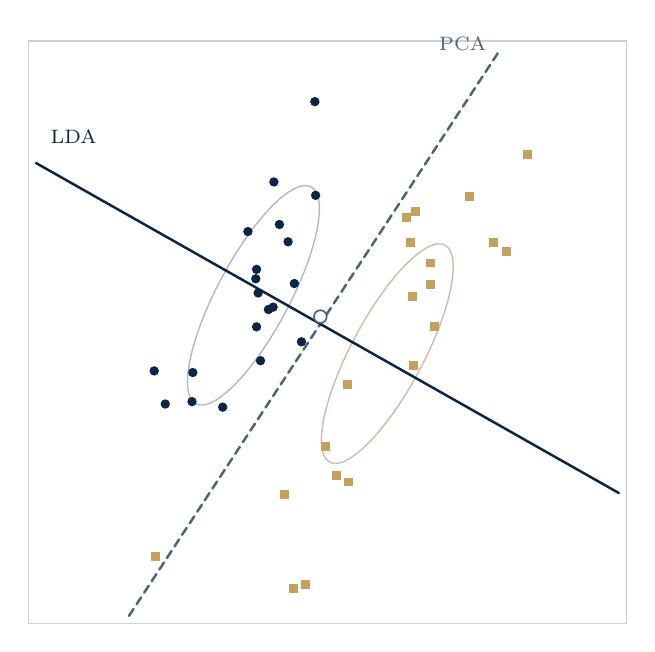
\begin{tikzpicture}[x=1cm,y=1cm,>=Latex,line cap=round]
  \draw[frame] (0,0) rectangle (7.6,7.4);
  \draw[steel!45,line width=0.5pt,rotate around={62:(2.86,4.17)}] (2.86,4.17) ellipse (1.56 and 0.46);
  \draw[gold!45,line width=0.5pt,rotate around={62:(4.56,3.43)}] (4.56,3.43) ellipse (1.56 and 0.46);
  \draw[steel,line width=0.9pt,densely dashed] (1.28,0.10) -- (6.00,7.30);
  \draw[navy,line width=0.9pt] (0.10,5.85) -- (7.50,1.66);
  \foreach \a/\b in {3.30/4.85, 3.64/6.63, 2.47/2.75, 2.92/4.20, 3.11/4.02,
                    2.08/2.82, 2.90/3.77, 2.95/3.34, 2.89/4.38, 3.47/3.58,
                    2.90/4.50, 3.05/3.99, 1.60/3.21, 2.79/4.98, 3.65/5.44,
                    3.12/5.61, 1.74/2.79, 3.19/5.07, 3.38/4.32, 2.09/3.19}{%
    \fill[cls1] (\a,\b) circle (1.7pt);}
  \foreach \a/\b in {4.89/3.28, 4.80/5.16, 4.05/3.04, 3.52/0.50, 1.62/0.85,
                    3.26/1.64, 4.86/4.84, 5.11/4.31, 4.88/4.16, 4.07/1.80,
                    5.91/4.84, 6.07/4.73, 4.92/5.24, 5.11/4.58, 5.60/5.42,
                    6.34/5.96, 3.37/0.45, 3.78/2.25, 5.16/3.77, 3.91/1.88}{%
    \fill[cls2] ($(\a,\b)+(-1.6pt,-1.6pt)$) rectangle ($(\a,\b)+(1.6pt,1.6pt)$);}
  \fill[white] (3.71,3.90) circle (2.3pt); \draw[steel,line width=0.6pt] (3.71,3.90) circle (2.3pt);
  \node[font=\scriptsize,text=steel,anchor=south east] at (5.94,7.16) {PCA};
  \node[font=\scriptsize,text=navy,anchor=south west] at (0.16,5.98) {LDA};
\end{tikzpicture}

\caption{同一份数据上的两个方向。两团数据沿 $62^\circ$ 方向被拉长，所以 PCA 选了这条「方差最大」的方向；而两类的中心几乎在水平方向上错开，LDA 选了近似垂直于拉长方向的那条。两者夹角 $86^\circ$，Fisher 准则的取值相差约 $480$ 倍（$0.010$ 对 $4.78$）。}
\label{fig:pca}
\end{figure}

图 \ref{fig:pca} 是一个极端的例子，但它说明的问题很普遍：\textbf{方差大的方向不一定是有用的方向}。在这份数据上，PCA 把全部精力花在了「摊得最开」的方向，而这个方向上两类几乎完全重叠。

\subsection{两类方法的差异}

\begin{center}
\small
\begin{tabular}{@{}p{2.5cm}p{5.2cm}p{5.2cm}@{}}
\toprule
\rowcolor{navy!7}
\tabhead & \tabhead PCA & \tabhead LDA\\
\midrule
优化目标 & 投影后总方差最大，即 $\bW\tp\bS_t\bW$ 的迹最大 & 投影后类间/类内之比最大，见 \eqref{eq:ldaK}\\[3pt]
是否用标签 & 不用，无监督 & 用，有监督\\[3pt]
维数上限 & $\min(D,N)$ & $\min(K-1,D)$\\[3pt]
典型用途 & 压缩、去噪、可视化 & 分类前的降维、可视化\\[3pt]
失效场景 & 判别信息藏在低方差方向 & 类内散布奇异、类别形状差异大\\
\bottomrule
\end{tabular}
\end{center}

维数上限这一条值得单独说。PCA 最多能取到 $D$ 维（受样本数限制），因为它对方向没有偏好；LDA 最多只有 $K-1$ 维，因为再多也没有判别信息可用（\S3.5）。所以当 $D$ 很大而 $K$ 很小时，LDA 的降维是\emph{本质性}的——它把 $D$ 维压到 $K-1$ 维，而且这 $K-1$ 维包含了全部分类所需的信息。

\begin{add}[能不能先 PCA 再 LDA]
可以，而且在实际问题里很常见。当 $D$ 很大（比如图像）导致 $\bS_w$ 奇异时，先用 PCA 把维数降到 $D'<N-K$，再在 $D'$ 维上做 LDA，是一种标准的补救手段（\S6.5 第 2 条）。

但要清楚这样做的代价：PCA 阶段是无监督的，它可能已经把判别信息丢掉了。如果先验地知道判别信息集中在高方差方向，这个做法没问题；否则应优先考虑正则化的 LDA（给 $\bS_w$ 加岭），而不是盲目先降维。
\end{add}

% ============================================================
%  第 6 节
% ============================================================

\section{算法实现、校验与适用条件}\label{sec:impl}

\subsection{算法步骤}

把前面的推导整理成可以直接实现的形式。输入是数据矩阵 $\bX\in\R^{N\times D}$ 与标签 $\by$，输出是投影矩阵 $\bW$、类均值、类先验。

\begin{enumerate}[label=\textbf{Step \arabic*.},leftmargin=4.2em,itemsep=0.35em]
  \item \textbf{算类统计量}：$N_c$、$\bar\bx_c$、$\bar\bx$。
  \item \textbf{算两个散布矩阵}：$\bS_w=\sum_c\sum_{i:y_i=c}(\bx_i-\bar\bx_c)(\bx_i-\bar\bx_c)\tp$，$\bS_b=\sum_c N_c(\bar\bx_c-\bar\bx)(\bar\bx_c-\bar\bx)\tp$。
  \item \textbf{Cholesky 分解} $\bS_w=\bL\bL\tp$（要求 $\bS_w$ 正定）。
  \item \textbf{对称化}：构造 $\bM=\bL^{-1}\bS_b\bL^{-\top}$，对它做 \texttt{eigh} 得特征值 $\lambda_k$ 与特征向量 $\bv_k$。
  \item \textbf{回代}：$\bW=\bL^{-\top}[\bv_1,\dots,\bv_d]$，自动满足 $\bW\tp\bS_w\bW=\bI_d$。
\end{enumerate}

第 4 步的 $\bM$ 是实对称的（$\bS_b$ 对称，$\bL^{-1}$ 合同变换保持对称），所以可以用 \texttt{eigh} 而不是 \texttt{eig}——前者返回实特征值、正交特征向量，且更稳定。

\begin{add}[为什么不直接对 $\bS_w^{-1}\bS_b$ 做特征分解]
因为它\emph{不对称}。不对称矩阵的特征向量一般不正交，也不满足 $\bW\tp\bS_w\bW=\bI_d$；数值上还要求逆，$\bS_w$ 接近奇异时误差会放大。白化之后问题变成一个对称矩阵的特征分解，既稳又快。
\end{add}

\subsection{参考实现}

下面这段代码只依赖 NumPy，二十行左右，可直接跑。

\begin{center}
\small
\begin{minipage}{0.94\textwidth}
\begin{verbatim}
import numpy as np

def lda_fit(X, y, d=None):
    classes, yi = np.unique(y, return_inverse=True)
    K, D = len(classes), X.shape[1]
    Nc = np.bincount(yi, minlength=K).astype(float)
    means = np.stack([X[yi == c].mean(0) for c in range(K)])   # (K, D)
    xbar = Nc @ means / Nc.sum()
    Xc = X - means[yi]                       # center by own class mean
    Sw = Xc.T @ Xc                           # (D, D)
    dmu = means - xbar
    Sb = (dmu * Nc[:, None]).T @ dmu         # (D, D)
    L = np.linalg.cholesky(Sw)
    M = np.linalg.solve(L, Sb)
    M = np.linalg.solve(L, M.T).T            # L^-1 Sb L^-T
    ev, V = np.linalg.eigh((M + M.T) / 2)
    order = np.argsort(ev)[::-1]
    d = min(K - 1, D) if d is None else d
    W = np.linalg.solve(L.T, V[:, order[:d]])   # W' Sw W = I
    return W, ev[order[:d]], means, Nc / Nc.sum()

def lda_predict(X, W, means, prior):
    d2 = ((X[:, None, :] @ W - means @ W) ** 2).sum(-1)
    return np.argmin(d2 - 2 * np.log(prior), axis=1)
\end{verbatim}
\end{minipage}
\end{center}

预测阶段只需要 $\bW$、类均值与先验；若要算完整的判别函数 $\delta_c$，还得保留 $\bS_w$（或它的 Cholesky 因子）以构造线性系数 $\bS_w^{-1}\bar\bx_c$。

\subsection{数值校验}

光看代码跑通不算数，得逐条对上理论。表 \ref{tab:verify} 是在 $K=4$、$D=10$、各类 $60/40/30/50$ 个样本、共享协方差的数据上做的检查（NumPy 2.4.2，固定随机种子，$N=180$）。

\begin{table}[htbp]
\centering
\small
\caption{LDA 实现的性质校验（固定种子，非泛化性能评估）}
\label{tab:verify}
\begin{tabular}{@{}p{8.4cm}l@{}}
\toprule
\rowcolor{navy!7}
\tabhead 检查项 & \tabhead 结果\\
\midrule
$\bS_w+\bS_b=\bS_t$ 的最大偏差 & $2.8\times10^{-13}$\\
$\rank(\bS_b)$ / 非零广义特征值个数 & $3=K-1$ / 恰 $3$ 个\\
$\bW\tp\bS_w\bW-\bI_d$ 的最大元素 & $5.6\times10^{-16}$\\
$\bW\tp\bS_b\bW$ 的非对角元最大绝对值 & $1.2\times10^{-15}$\\
$\sum_k\lambda_k$ 与 $\tr(\bW\tp\bS_b\bW)$ & $17.41$ / $17.41$\\
$2$ 万个随机 $\bS_w$-正交 $\bW$ 的最大迹 & $14.15<17.41$\\
$2$ 万个随机方向的最大 $J$ & $8.46<9.90$\\
投影最近质心 vs 马氏最近质心（$d=3$） & $180/180$ 一致\\
同上（$d=2$） & $177/180$\\
同上（$d=1$） & $135/180$\\
训练准确率（$d=3$ / $d=2$ / $d=1$） & $99.4\%$ / $97.8\%$ / $75.6\%$\\
\bottomrule
\end{tabular}
\end{table}

前五行是恒等式，偏差都在机器精度量级，说明推导与实现一致。第六、七行是\emph{随机搜索}的对照：在所有满足约束的 $\bW$ 里随机采两万个，没有一个超过特征值解，这与「$\sum_k\lambda_k$ 是约束下的上界」吻合（但随机搜索本身不构成证明）。最后三行说明一件实践中的事：\textbf{把维数从 $K-1$ 砍到 $1$，准确率掉了二十多个百分点}——降维可视化好看，但不能拿它当完整 LDA 的决策依据。

\subsection{复杂度}

\begin{itemize}
  \item 训练：算两个散布矩阵 $O(ND^2)$，Cholesky $O(D^3)$，对称特征分解 $O(D^3)$，总计 $O(ND^2+D^3)$；空间 $O(D^2)$。
  \item 预测：单样本 $O(Dd)$（算 $d$ 个投影坐标再比 $K$ 个距离）；整批 $O(N_{\text{new}}Kd)$。
  \item 若只要判别函数而不降维，预测是 $O(KD)$，与 $d$ 无关。
\end{itemize}

当 $D$ 远大于 $N$ 时，$O(D^3)$ 会成为瓶颈，此时通常先做一次 PCA 或随机投影把 $D$ 压下来——但要注意 \S5 说的信息损失问题。

\subsection{假设与失效场景}

LDA 的公式很短，但它的前提不短。下面七条，按在实践里踩坑的频率排序。

\paragraph{1. 共享协方差。}$\bS_w$ 把所有类的协方差揉成一份，等价于假设各类「同形同尺度」。若各类差异大（比如某一类特别松散），这份平均会被大类或大散布类主导，方向偏向它。

\emph{诊断}：逐类看 $\lvert\bS_c\rvert$ 与 $\tr(\bS_c)$ 的量级。
\emph{处理}：改用 QDA，或先对每类白化再合并，或用收缩估计把 $\bS_c$ 往 $\bS_w$ 拉。

\paragraph{2. $\bS_w$ 奇异。}$\bS_w$ 的秩至多 $N-K$。当 $N-K<D$（小样本高维）或特征强共线时，$\bS_w$ 不满秩，Cholesky 直接失败、$\bS_w^{-1}$ 不存在。

\emph{处理}：加岭 $\bS_w\leftarrow\bS_w+\lambda\bI$（$\lambda>0$ 是正则强度，与特征值记号无关），或先用 PCA 降到 $D'<N-K$ 维。$\lambda\to\infty$ 时 $\bS_w+\lambda\bI\approx\lambda\bI$，方向退化成 $\bS_b$ 的主特征向量——也就是「只看类中心差的 PCA」。

\paragraph{3. 对特征尺度敏感。}$\bS_w$ 与 $\bS_b$ 都按原始单位计算，量纲大的特征会主导特征值。把「米」换成「毫米」，判别方向就会变。

\emph{处理}：先标准化。但标准化参数只能来自训练集——这条与上一讲的「泄漏」是同一个问题。

\paragraph{4. 对离群点敏感。}均值与协方差都是非鲁棒统计量，一个离群点就能显著改变 $\bS_b$ 与 $\bS_w$。

\emph{处理}：稳健标准化（用中位数与四分位距代替均值与标准差），或先剔除可疑点，或改用基于秩的方法。

\paragraph{5. 类别不平衡。}$\bS_b$ 里的 $N_c$ 让大类主导方向，$\bS_w$ 亦然；先验项 $\log\hat\phi_c$ 又让大类更容易被选中。若关心宏平均或 F1 而非总体准确率，这套默认行为是错的。

\emph{处理}：改用等权 $\bS_b$ 与等先验，或对损失加权。

\paragraph{6. 数据泄漏。}$\bS_w$、$\bS_b$、$\bar\bx_c$ 都是训练集统计量。用全量数据估完再划分训练/测试，评估会虚高。

\emph{处理}：把「估均值与散布」当成模型的一部分，放进交叉验证的每一折里。

\paragraph{7. 不要把它当非线性方法。}类别边界由超平面切出。异或型数据、同心球型数据，LDA 必然失败——这与共享协方差的 GDA 失败的方式完全相同。

\emph{诊断}：把数据投到前两个判别方向上画散点，若两类在二维平面上仍然犬牙交错，说明线性边界不够用。
\emph{处理}：加特征（平方项、交互项）、用核 LDA，或换非线性模型。

\begin{warn}[一个常见误解]
「LDA 假设数据服从正态分布」这句话不完全对。LDA 的\emph{判别函数}只需要各类的均值与共享协方差，不要求正态；正态假设是在推导「$\delta_c$ 是后验对数」时才用到的。换句话说，\textbf{即使数据不正态，$\hat\bw\propto\bS_w^{-1}(\bar\bx_1-\bar\bx_2)$ 仍是一个合理的方向}，只是它不再有「最优贝叶斯分类器」的解释。
\end{warn}

% ============================================================
%  第 7 节
% ============================================================

\section{小结}

\subsection{五个要点}

\begin{enumerate}[label=\textcolor{navy}{\bfseries\arabic*.},leftmargin=2.3em,itemsep=0.55em]
  \item \textbf{LDA 就是一个方向加一个阈值。}方向由 $\bS_w^{-1}(\bar\bx_1-\bar\bx_2)$ 给出，阈值放在两类得分的中点（先验不等时平移）。
  \item \textbf{这个方向不是中心连线。}$\bS_w^{-1}$ 先把空间白化，让所有方向的类内散布都变成 $1$，再在白化空间里沿中心连线看——几何上等价，直觉上完全不同。
  \item \textbf{多类时是一个广义特征值问题。}$\bS_b\bW=\bS_w\bW\bLambda$，取前 $d$ 个特征向量并归一化成 $\bW\tp\bS_w\bW=\bI_d$。
  \item \textbf{最多 $K-1$ 维。}$\rank(\bS_b)\le K-1$，因为类中心偏差的加权和为零。这个上限与 $\rank(\bS_w)\le N-K$ 是两个独立的上限，管的事情不同。
  \item \textbf{它与 GDA 是同一个模型。}$\bSigma=\bS_w/N$，共享协方差的高斯假设恰好生产出线性判别函数。松开共享假设就得到 QDA。
\end{enumerate}

\subsection{知识结构}

\begin{figure}[htbp]
\centering
% ---- 插图：fig-map ----
\begingroup
\providecommand{\ttl}{\bfseries\sffamily\color{navy}}
\providecommand{\fml}{\scriptsize\color{navy!88}}
\scalebox{0.98}{%
\begin{tikzpicture}[
  box/.style={draw=navy!55,fill=navy!3,minimum width=2.55cm,minimum height=1.78cm,
    align=center,inner sep=2pt,sharp corners,line width=0.5pt},
  ar/.style={->,navy!60,line width=0.6pt},
]
\node[box] (b1) at (1.35,0) {{\ttl 数据}\\[1pt]{\fml $\bX\in\R^{N\times D}$}\\[0pt]{\fml $y\in\{1,\dots,K\}$}};
\node[box] (b2) at (4.30,0) {{\ttl 类内/类间}\\[1pt]{\fml $\bS_w,\ \bS_b$}\\[0pt]{\fml $\bS_t=\bS_w+\bS_b$}};
\node[box] (b3) at (7.25,0) {{\ttl 方向}\\[1pt]{\fml $\bS_b\bW=\bS_w\bW\bLambda$}\\[0pt]{\fml $d\le K-1$}};
\node[box] (b4) at (10.20,0) {{\ttl 判别}\\[1pt]{\fml $\delta_c(\bx)$ 线性}\\[0pt]{\fml 超平面边界}};
\node[box] (b5) at (13.15,0) {{\ttl 概率}\\[1pt]{\fml 共享协方差高斯}\\[0pt]{\fml $\bSigma=\bS_w/N$}};

\draw[ar] (b1) -- (b2);
\draw[ar] (b2) -- (b3);
\draw[ar] (b3) -- (b4);
\draw[ar] (b4) -- (b5);
\draw[<->,navy!45,line width=0.55pt,densely dashed] (b2.north) to[bend left=22] (b5.north);

\node[draw=navy!25,fill=white,align=center,font=\footnotesize,inner sep=5pt]
  at (7.25,-1.58)
  {几何：投影 + 阈值 \quad $\cdot$ \quad 概率：贝叶斯 + 高斯 \quad $\cdot$ \quad 降维：有监督的 PCA};
\end{tikzpicture}}
\endgroup

\caption{本讲的知识地图。横向是一条流水线：从数据到散布矩阵，到方向，到判别函数，最后到概率解释。中间那条弧线是本讲的主旨——几何与概率两条路，终点是同一个模型。}
\label{fig:map}
\end{figure}

\subsection{后续内容}

这一讲停在「线性边界」上。往下走有三条路：

\begin{itemize}
  \item \textbf{换成概率输出}。LDA 只能给类别；若想要 $p(y=1\mid\bx)$，就走向逻辑回归。它的边界仍是线性的，但不再假设类条件分布（\S4.5）。
  \item \textbf{换成非线性边界}。QDA 是最省事的一步（二次曲面）；再往前是核方法——把 $\bx$ 映射到高维，让线性边界在原空间里变成曲线。
  \item \textbf{换成「最大间隔」的视角}。支持向量机不问「类内多散」，只问「边界离最近的点有多远」。这是另一种完全不同的判据，但同样落在 $\bw\tp\bx+b$ 这个骨架上。
\end{itemize}

% ============================================================
%  习题
% ============================================================

\clearpage
\section*{习题}
\addcontentsline{toc}{section}{习题}
\markboth{习题}{}
\setlength{\parskip}{0.62em}

\subsection*{A 组 · 基础}

\noindent\textbf{A1.} 用表 \ref{tab:iris} 的数据，手算 $\bar\bx_1,\bar\bx_2$ 与 $\bS_w$，验证 $\det\bS_w=0.3654$。

\noindent\textbf{A2.} 接着上题，算出 $\bS_w^{-1}(\bar\bx_2-\bar\bx_1)$ 并归一化，验证它等于 $(0.622,\,0.783)\tp$，与横轴夹角 $51.6^\circ$。

\noindent\textbf{A3.} 计算十个样本的投影得分 $z=\hat\bw\tp\bx$，验证两类得分区间分别是 $[3.41,4.44]$ 与 $[5.30,5.40]$，并算出中点阈值。

\noindent\textbf{A4.} 对 A3 的数据，若先验改为 $\hat\phi_1:\hat\phi_2=0.6:0.4$，阈值移到哪里？判定结果有没有变化？

\noindent\textbf{A5.} 验证 $\bS_t=\bS_w+\bS_b$：用表 \ref{tab:iris} 的数据算出三个 $2\times2$ 矩阵，逐元素核对。

\subsection*{B 组 · 提高}

\noindent\textbf{B1.} 证明：只要 $\bS_w$ 正定，$J(\bw)$ 在 $\bw\propto\bS_w^{-1}(\bar\bx_1-\bar\bx_2)$ 处取到全局最大值，且最大值等于 $(\bar\bx_1-\bar\bx_2)\tp\bS_w^{-1}(\bar\bx_1-\bar\bx_2)$（二分类、$\bS_b$ 用不带系数的写法）。

\noindent\textbf{B2.} 证明 $\bS_b$ 的秩不超过 $K-1$，并构造一个例子说明等号可以取到、也可以取不到。

\noindent\textbf{B3.} 证明：在约束 $\bW\tp\bS_w\bW=\bI_d$ 下，
$\tr(\bW\tp\bS_b\bW)\le\sum_{k=1}^{d}\lambda_k$，其中 $\lambda_k$ 是 $\bS_w^{-1}\bS_b$ 的广义特征值（降序）。

\noindent\textbf{B4.} 设 $\bS_w=\bI$，$\bS_b$ 如 \eqref{eq:sb}。写出此时的 $\hat\bw$，并解释它与「最近质心分类器」的关系。

\noindent\textbf{B5.} 证明：若两类先验不等，则 \eqref{eq:boundary} 给出的边界沿 $\bS_w^{-1}(\bar\bx_2-\bar\bx_1)$ 方向平移了 $\log(\hat\phi_1/\hat\phi_2)$ 除以 $\norm{\bS_w^{-1}(\bar\bx_2-\bar\bx_1)}$ 的距离。

\subsection*{C 组 · 动手}

\noindent\textbf{C1.} 实现 \S6.2 的代码，在两类鸢尾数据上验证 $J(\hat\bw)=7.40$；再随机采 $10^4$ 个单位方向，确认没有哪个方向的 $J$ 更大。

\noindent\textbf{C2.} 生成 $K=3$、$D=2$、每类 $50$ 个样本的三团高斯数据，做 LDA，把两个判别方向画在散点上，并把投影后的二维散点画在右侧。观察三类是否被分开。

\noindent\textbf{C3.} 在同一份数据上分别做 PCA 与 LDA，画出两个方向。构造一份数据使两者夹角超过 $60^\circ$，并解释为什么。

\noindent\textbf{C4.} 取 $D=200$、$N=60$ 的高维小样本数据，直接调用 \texttt{np.linalg.cholesky} 会报错。改用 $\bS_w+\lambda\bI$，画出 $\lambda$ 从 $10^{-4}$ 到 $10^{2}$ 时首个判别方向与「$\bS_b$ 主特征向量」的夹角变化。

\subsection*{提示}

\begin{itemize}[itemsep=0.2em]
  \item \textbf{A1}：先算两类均值，再对每个样本减去本类均值，最后把十个外积相加。
  \item \textbf{A4}：阈值是 $\hat\bw\tp\frac{\bar\bx_1+\bar\bx_2}{2}+\log\frac{0.6}{0.4}$，注意第二项是纯数，要加在 $z$ 上。
  \item \textbf{B1}：用瑞利商，或直接用 Cauchy--Schwarz 不等式。
  \item \textbf{B2}：等号取到的例子：$K$ 个类中心构成正单纯形；取不到的例子：两个类中心重合。
  \item \textbf{B3}：把 $\bW$ 用 $\bS_w$-标准正交基展开，逐项用 $\lambda_k$ 放缩。
  \item \textbf{B5}：把 \eqref{eq:boundary} 写成 $\bw\tp(\bx-\bx_0)=0$ 的形式，读出 $\bx_0$。
  \item \textbf{C4}：$\lambda$ 很大时 $\bS_w+\lambda\bI\approx\lambda\bI$，方向趋于 $\bS_b$ 的主特征向量。
\end{itemize}

% ============================================================
%  附录
% ============================================================

\appendix
\renewcommand{\thesection}{\Alph{section}}

\section{公式速查}

\subsection*{A.1 多元正态与马氏距离}

$D$ 维正态密度
\begin{equation}
  \mathcal{N}(\bx;\bmu,\bSigma)=\frac{1}{(2\pi)^{D/2}\lvert\bSigma\rvert^{1/2}}
  \exp\Bigl[-\tfrac12(\bx-\bmu)\tp\bSigma^{-1}(\bx-\bmu)\Bigr].
\end{equation}
指数上那个二次型就是\textbf{马氏距离的平方}。它与欧氏距离的差别是「先把各方向按标准差归一化，再量距离」——这正是白化的作用。

\subsection*{A.2 三个常用的矩阵事实}

\begin{enumerate}[label=(\arabic*),leftmargin=2.0em]
  \item \textbf{合同变换保秩}：$\rank(\bA\bB)\le\min(\rank\bA,\rank\bB)$，故 $\rank(\bS_b)=\rank(\sum_c N_c\bdelta_c\bdelta_c\tp)\le K-1$。
  \item \textbf{相似变换保特征值}：$\bA\bB$ 与 $\bB\bA$ 的非零特征值相同（$\bA$ 可逆时完全相同）。这就是 $\bS_w^{-1}\bS_b$ 与 $\bS_w^{-1/2}\bS_b\bS_w^{-1/2}$ 特征值一致的依据。
  \item \textbf{迹的循环性}：$\tr(\bA\bB)=\tr(\bB\bA)$。约束优化里把 $\tr(\bLambda\tp\bW\tp\bS_w\bW)$ 整理成 $\tr(\bW\tp\bS_w\bW\bLambda)$ 就靠它。
\end{enumerate}

\subsection*{A.3 瑞利商}

对实对称矩阵 $\bA$，函数 $R(\bu)=\dfrac{\bu\tp\bA\bu}{\bu\tp\bu}$ 的最大值等于 $\bA$ 的最大特征值，在对应特征向量处取到；最小值对应最小特征值。这是 \S2.4「第二条路」的全部依据。

\subsection*{A.4 记号对照}

\begin{center}
\small
\begin{tabular}{@{}lll@{}}
\toprule
\rowcolor{navy!7}
\tabhead 本讲 & \tabhead 常见别名 & \tabhead 说明\\
\midrule
$\bS_w$ & $S_w$、within-class scatter & 类内散布（平方和）\\
$\bS_b$ & $S_B$、between-class scatter & 类间散布（带 $N_c$ 权重）\\
$\bS_t$ & $S_T$、total scatter & 总散布\\
$\delta_c(\bx)$ & discriminant function & 判别函数\\
$\bSigma$ & pooled covariance & 共享协方差（$=\bS_w/N$）\\
\bottomrule
\end{tabular}
\end{center}

\section{延伸阅读}

\begin{enumerate}[label={[\arabic*]},leftmargin=2.6em,itemsep=0.7em]
  \item R. A. Fisher. The use of multiple measurements in taxonomic problems.
  \emph{Annals of Eugenics}, 7(2):179--188, 1936.\\[1pt]
  {\footnotesize\color{steel}LDA 的原始文献，用的正是鸢尾花数据。文字古朴，思路清晰。}

  \item C. M. Bishop. \emph{Pattern Recognition and Machine Learning}. Springer, 2006.\\[1pt]
  {\footnotesize\color{steel}第 4.1--4.3 节：判别函数、Fisher 判别、概率生成模型。图 4.6 与本讲图 \ref{fig:proj} 是同一种画法。}

  \item T. Hastie, R. Tibshirani, J. Friedman. \emph{The Elements of Statistical Learning}, 2nd ed. Springer, 2009.\\[1pt]
  {\footnotesize\color{steel}第 4.3 节：LDA 与 QDA 的比较、正则化判别分析。对「共享协方差」的讨论最清楚。}

  \item K. Fukunaga. \emph{Introduction to Statistical Pattern Recognition}, 2nd ed. Academic Press, 1990.\\[1pt]
  {\footnotesize\color{steel}第 3 章：散布矩阵与特征提取的系统处理，含 $K-1$ 维上限的多种证明。}

  \item 周志华. 《机器学习》. 清华大学出版社, 2016.\\[1pt]
  {\footnotesize\color{steel}第 3.4 节：LDA 的广义特征值推导，中文表述最简洁的一本。}
\end{enumerate}

\vspace{1.0em}
\begin{flushright}
{\color{navy!25}\rule{3.2cm}{0.5pt}}\\[5pt]
{\kaishu\footnotesize\color{steel}CyArk}
\end{flushright}

\end{document}
